\chapter{Design} \label{chap:design}

%\version{v1.10.2015}

\section*{}
Indus Bazar is implemented in a scalable, modular B2B marketplace application where the user-friendly mobile interface, business logic on the server, and the persistent data layer are cleanly separated. Its architecture is based on a three-tier model with Flutter used as the cross-platform frontend, Appwrite as the Backend-as-a-Service (BaaS) layer, and a series of Node.js serverless cloud functions, performing sensitive functions like processing payments, deducting stocks, and sending push notifications. Security, real-time responsiveness, and role based access control of Customer and Sellers were major considerations during the design process.


\section{System Architecture}
Indus Bazar has a 3-Tier Architecture that provides a scalable, maintainable and secure B2B marketplace experience. The three layers clearly distinguish between presentation issues and business logic and data persistence, allowing each layer to be scaled separately and easily extended with new features over time.

\subsection{3-Tier Architecture Overview}

The system is based upon a 3-Tier Architecture:

\begin{enumerate}
    \item \textbf{Presentation Tier (Flutter Mobile App)} – The cross-platform Flutter application will be the one to handle all the end-user interfaces of both Customers and Sellers. Important screens are authentication (login, signup, email verification, password reset), a role-based home dashboard, product browsing and product detail views, cart and checkout flow, order tracking, RFQ (Request for Quotation) workflow, real-time chat, seller product and order management, and the review system. State is reactively handled with the Riverpod (hooks riverbed) library to have specific providers of authentication, products, cart, orders, RFQs, chat and payment.

    \item \textbf{Application Tier (Appwrite BaaS + Node.js Cloud Functions)} - Appwrite offers authentication (email / password sessions with email verification required), a no-SQL document database, file storage, where product images are located, and server-side permissions through Row-Level Security. Eight serverless functions in Node.js that run on the Appwrite service are in charge of activities needing elevated privileges or external API requests: create-payment-intent and process-order to Stripe payment and atomic stock deduction; seller-order-actions to seller-side RLS bypass; rfq-actions to RFQ lifecycle management; send-chat-notification, send-order-notification, and send-rfq-notification

    \item \textbf{Data Tier (Appwrite Collections \& Storage)} - All data is stored in the NoSQL document store of Appwrite, and it is structured into thirteen collections, such as user roles, products, cart, orders, addresses, seller profiles, reviews, product stats, conversations, messages, rfqs, and rfq quotes. Binary (product images, review images) are stored in an Appwrite Storage bucket (product\_images). Firebase Cloud Messaging only delivers push-notifications; it does not have any Firebase database.
\end{enumerate}

\begin{figure}[H]
\centering
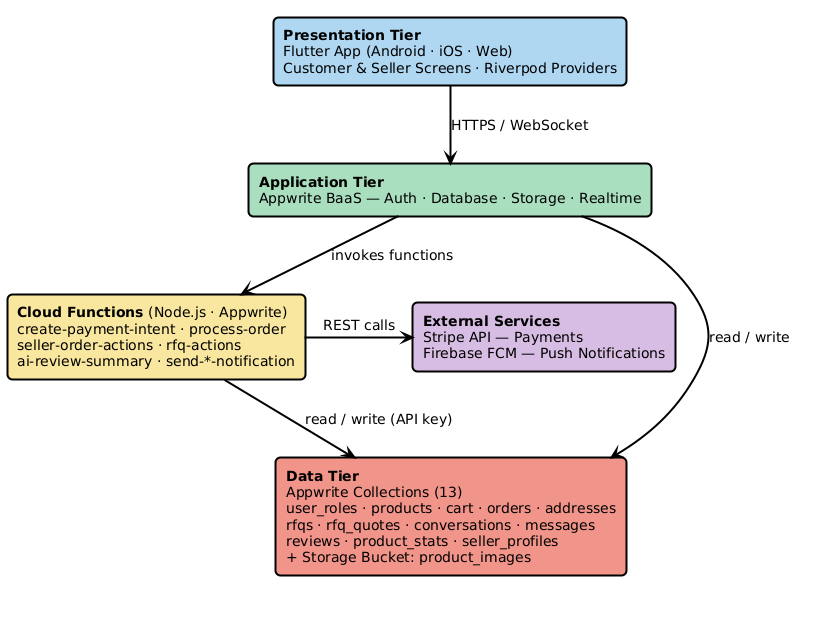
\includegraphics[width=1.1\textwidth]{figures/pictures project/Architecture.png}
\caption{Indus Bazar 3-Tier System Architecture}
\label{fig:system_architecture}
\end{figure}

The architectural illustration in Figure \ref{fig:system architecture} depicts three-tier design of Indus Bazar. Presentation Tier (Flutter app) talks to the Application Tier (Appwrite cloud hosted at fra.cloud.appwrite.io with its serverless functions) via HTTPS. The serverless functions make calls to the Stripe Payments API to create payment intent and Firebase Cloud Messaging API to deliver push notifications. The Data Tier (Appwrite document collections and Storage) can only be accessed via the Appwrite SDK, and all access control policies are implemented on the server-side.

\section{Design Constraints}
This part describes the main constraints and criteria which affect design and development of the Indus Bazar B2B Marketplace.

\subsection{Technical Constraints}
\begin{itemize}
    \item Flutter application is cross-platform (Android, iOS, Web), meaning it has cross-platform requirements on both UI and plugins (e.g. Stripe flutter\_stripe package does not initialise on Web).
    \item Chat Real-time chat needs Appwrite Realtime subscriptions; thus, the message one-to-many collection is designed to allow document events to be streamed in real-time.
    \item All Stripe payments need server-initiated through a cloud function to secure the Stripe secret key; the client simply receives a clientSecret and completes the payment sheet on-locally.
    \item Image uploads: Appwrite Storage using file\_picker with file\_picker and file size and MIME-type validation on the client and at the bucket level.
\end{itemize}

\subsection{Security \& Privacy Constraints}
\begin{itemize}
    \item Email verification This is required: the AppWrapper widget will not allow any navigation to home screens unless isEmailVerified is true; unverified users will always be redirected to the EmailVerificationScreen.
    \item Appwrite Row-Level Security (RLS) document permissions are configured at document creation, and are limited to the owning user(s), restricting read and write access. The seller functions which have to circumvent RLS (e.g., inspecting another users order to update its status) are only carried out within server-side cloud functions with an Appwrite API key.
    \item Stripe publishable key This is the only Stripe credential that is stored in the client-side; the secret key does not exit the create-payment-intent cloud function environment.
    \item Push notification FCM tokens are created in appwrite as a push target child of the authenticated user and unregistered on logout to avoid leakage of notifications.
\end{itemize}

\subsection{Operational Constraints}
\begin{itemize}
    \item The backend is automatically scaled on Appwrite Cloud (Frankfurt region); it does not need an on-premises infrastructure.
    \item cold-starting cloud functions on-demand; latency-sensitive routes (e.g., payment intent) Java lightweight Node.js runtimes to maintain decent response times.
    \item The deduction of product stock at the checkout is managed atomically within the process-order cloud function to avoid overselling when there are concurrent orders.
    \item The RFQ expiry policy (quotes automatically expire on deadline) is implemented with the rfq-actions function to keep the data consistent without client-side timers.
\end{itemize}

\section{Design Methodology}

A mix of Modular Design and Agile Prototyping was used to create Indus Bazar to make it flexible, separate concerns, and deliver working features as the project progressed.

\subsection{Modular Design}

The application itself is broken down into self-contained modules, each containing its own screens, providers, services and models. This separation permits independent development and testing of each domain:

\begin{itemize}
    \item \textbf{Authentication Module} -- Registration, login, email verification, password reset and role assignment (Customer / Seller).
    \item \textbf{Product Catalogue Module} -- Product listing, category filtering and search, product detail, tiered pricing display, multi-image gallery and seller product management (add/edit/deactivate).
    \item \textbf{Cart \& Checkout Module} -- Cart management, quantity sensitive tiered price recalculation, address selection and Stripe payment sheet integration.
    \item \textbf{Order Management Module} -- Customer order history; order status tracking; seller order dashboard with order status progression (pending $\to$ confirmed $\to$ shipped $\to$ delivered).
    \item \textbf{RFQ (Request for Quotation) Module} -- Customer RFQ creation including specifications and target price range; open RFQ marketplace including sellers; sellers submit quote; customer accepts quote and makes payment.
    \item \textbf{Chat \& Messaging Module} -- Per-product chat and messaging between Customer and Seller: Appwrite Realtime! badges to indicate unread messages, and file attaching support.
\end{itemize}

\subsection{Agile Prototyping}
The development was planned as four sprints. At the end of every sprint, there was an incremental functional, testable portion of the application.

\begin{itemize}
    \item \textbf{Sprint 1}: Authentication (registering, logging into, verifying email, role-based routing) and Product Catalogue (browsing, product detail, tiered pricing, seller product management).
    
    \item \textbf{Sprint 2}: Cart Stripe payment integration (cloud functionality + payment sheet), Customer and Seller Order Management and Address management.
    
    \item \textbf{Sprint 3}: RFQ system (creation, open marketplace, quote submission and acceptance, RFQ-based payment) and real-time Chat \& Messaging with Appwrite Realtime.
    
    \item \textbf{Sprint 4}: Review system, verified-purchase enforcement, AI-generated review summaries, Seller Profile management, and FCM push notification delivery of all key events.
\end{itemize}

Each sprint involved planning, development, testing, and feedback to have interdependency among modules sorted out early and the final system was able to satisfy all functional requirements.

\section{System Activity Diagram}

The general workflow of Indus Bazar is described through activity diagrams, which illustrate the end-to-end processes of its two main user roles, Customer and Seller, starting with the process of logging in until the final stages of completing the commercial transactions. These charts are graphical representations of the flow of activity, decision-making and system feedback to perform different functionalities of the platform. The activity diagrams demonstrate the way users make contact with the system and data movement between the modules are well established thus creating clear understanding of the processes of operation. They emphasize the rational flow of actions, activities simultaneity, and conditional branching that takes place in the real-time operations in the B2B marketplace.

\subsection{Customer Activity Diagram}

To the Customer, the activity diagram illustrates user authentication, product discovery, viewing product details, RFQs, communicating with sellers over real-time chat, adding items to the shopping cart, checkout, and secure payments with Stripe, and order status tracking. It also incorporates the optional directions towards negotiating quotes, reviewing products, and reading AI-generated review summaries. The workflow starts with customer registration/ log-in, then email verification where the customers are assured safe access to the platform. When authenticated, customers are able to view categorized listings of products, filter using advanced search filters and compare tiered pricing structures before they make purchase decisions. 

Figure \ref{fig:customer_activity_diagram} represents the overall end-to-end process of a registered customer in Indus Bazar B2B marketplace. This is done by registering a new user by entering his full name, email address, password, and Customer role. When registration is successful, an automatic verification email will be sent through Appwrite. The customer has to authenticate their email prior to access and the AppWrapper widget constantly checks the authentication status and blocks unverified users. Upon verification, the customer is redirected to Customer Home screen, the main center of all activities in the platform. There are two major procurement paths enabled in the Customer Home screen that are: \textbf{Direct Purchase} and \textbf{RFQ (Request for Quotation)}. Under the Direct Purchase route, a customer navigates through the product catalogue with search and filter options, looks through the product specifications, including tiered pricing, places an order by the required quantity, and adds to the cart. 

\begin{figure}[htbp]
\centering
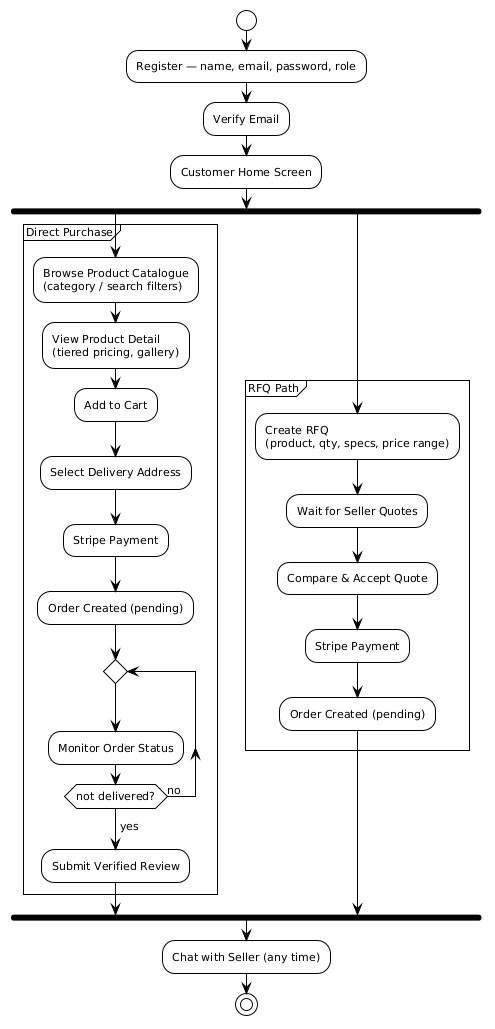
\includegraphics[width=0.72\textwidth]{figures/pictures project/Customer_Activity_Diagram.png}
\caption{Customer Activity Diagram}
\label{fig:customer_activity_diagram}
\end{figure}

The customer activity diagram in Figure \ref{fig:customer_activity_diagram} will help demonstrate the entire end to end process of a registered customer in the Indus Bazar B2B marketplace. This is done by registering a new user by entering his full name, email address, password, and Customer role. When registration is successful, an automatic verification email will be sent through Appwrite. The customer has to authenticate their email prior to access and the AppWrapper widget constantly checks the authentication status and blocks unverified users. Upon verification, the customer is redirected to Customer Home screen, the main center of all activities in the platform.

There are two major procurement paths enabled in the Customer Home screen that are: \textbf{Direct Purchase} and \textbf{RFQ (Request for Quotation)}. Under the Direct Purchase route, a customer navigates through the product catalogue with search and filter options, looks through the product specifications, including tiered pricing, places an order by the required quantity, and adds to the cart. At checkout, the customer verifies the shipping address and finalizes the payment safely with Stripe using credentials that are generated by the server. The system will automatically make the order, update inventory and send confirmation and push notifications on successful payment. The Orders screen allows customers to monitor the status of their orders in real time.

Bulk procurement or customized procurement is supported on the RFQ path. Customers place an RFQ with product requirements and quantities, location of delivery, specifications, and optional price ranges. The RFQ is posted to the market, and the sellers are allowed to make competitive bids. Customers read and compare the quotes received, pick the most appropriate offer and continue on the reliable Stripe payment flow. Once payment is confirmed, the system will create an order based on the accepted quotation and will shut-down the RFQ to additional bids to provide a smooth and transparent procurement process.


\subsection{Seller Activity Diagram}
To the Seller, the diagram describes the following activities: registration and verification of accounts, product listing and catalog, managing tiered pricing, RFQ responses, customer interaction in the chat system, receiving orders, updating order status, and delivery. It also emphasises administrative activities like tracking sales performance, handling quotations, and customer feedback. These charts also illustrate system-level processes of email verification, push notifications, secure payment processing, and automated order creation. Conditional flows, including the success or failure of a payment, the acceptance or rejection of an RFQ, and the confirmation or cancellation of an order are drawn using decision nodes.

Moreover, the activity diagrams have integrations with third-party services, such as Stripe to process secure payments, Appwrite to implement backend services and cloud functions, and Firebase Cloud Messaging (FCM) to implement real-time push notifications. These integrations guarantee a responsive, scalable and secure platform. The System Activity Diagrams can be used as a powerful reference resource by developers, stakeholders, and system analysts by offering the visual representation of user interactions and backend processes in a comprehensive manner. They enable system insight, authenticate functional requirements, and enable effective implementation, testing, and addition of the Indus Bazar B2B Marketplace in the future.
\begin{figure}[htbp]
\centering
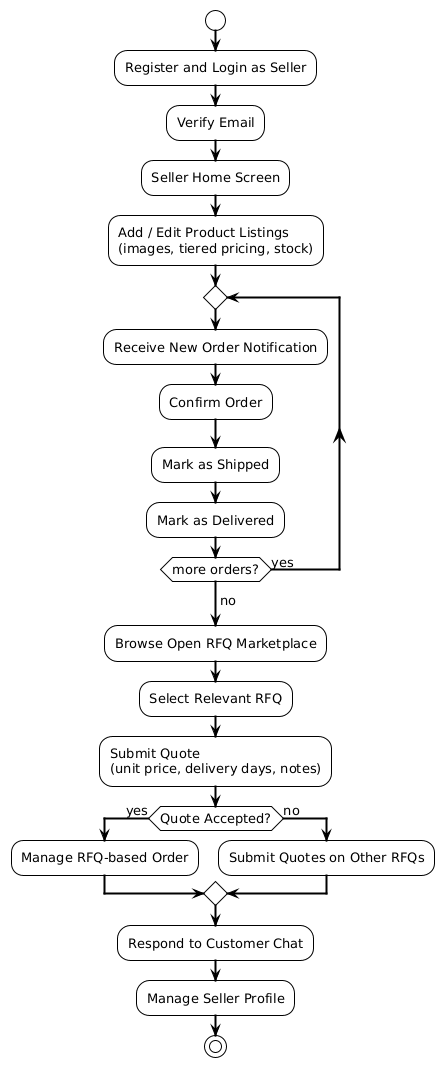
\includegraphics[width=0.61\textwidth]{figures/pictures project/Seller_Activity.png}
\caption{Seller Activity Diagram}
\label{fig:seller_activity_diagram}
\end{figure}

The seller activity diagram (Figure \ref{fig:seller_activity_diagram} presents the entire workflow a registered seller has in the Indus Bazar platform. The process starts with the registration and email verification, then the seller is redirected to the Seller Home, which is a main dashboard of all operations related to the sellers. Out of this hub there are two parallel streams of operation that the seller can be involved in either at the same time or alternately as per the business need.

At the stream Product and order management, the seller starts by developing and maintaining his or her product catalogue. The products listing contains a name, description, category, stock quantity, up to three images of the product uploaded to the Appwrite Storage, and a price structure based on tiers which enables the seller to provide lower unit prices with increased order volume a core aspect of B2B procurement. As soon as listings are active, the seller sees the customer orders that are coming in via the Seller Orders screen. Every new order will send out a push notification to the device of the seller, and no order will go undetected. The seller then completes each order by following the established lifecycle phases where receipt is established, the order is marked as shipped after dispatched and finally it is marked as delivered after successful handover that keeps the customer updated at every stage through automatic status updates.

Through the \textbf{RFQ Response} stream, the seller visits the open RFQ marketplace, which consolidates all the active Requests for Quotation placed by customers in the platform. The seller identifies RFQs associated with their product catalogue, examines specifications and target price range of the customer and sends a competitive quote, which includes unit price, total price, estimated delivery days and any other notes. When the customer accepts a quote made by the seller then an order is automatically generated and is handled by the same order lifecycle as direct purchases. The seller can also reply to customer messages at any stage of both streams using the integrated real time chat system and retain first person contact to be able to clarify product details or bargain. The seller is also able to access and update his or her public seller profile that will show his or her business name, city, contact details and aggregate rating aspects which directly affect buyer confidence and their buying choices.

\section{High Level Design}
High Level Design (HLD) displays the key building blocks of the Indus Bazar, interactions between them, and topology. The HLD does not include the specifics of implementation, but gives a bird-eye view of how the components of the system work together to provide B2B marketplace functionality.

\subsection{Component Diagram}
The Component Diagram will define the key software elements of Indus Bazar and interfaces with each other.

\begin{figure}[H]
\centering
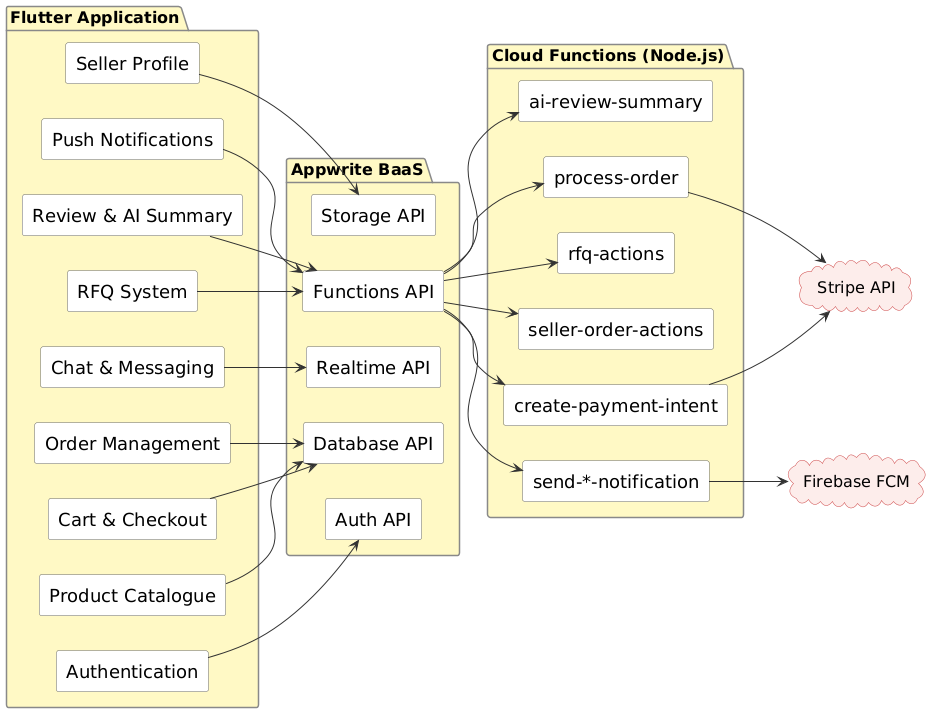
\includegraphics[width=1.0\textwidth]{figures/pictures project/component_diagram.png}
\caption{Component Diagram}
\label{fig:component_diagram}
\end{figure}

The component diagram in Figure \ref{fig:component_diagram} depicts the modular configuration of Indus Bazar. The Presentation Tier is comprised of the Flutter application that includes 9 logical sub-elements: Authentication, Product Catalogue, Cart / Checkout, Order Management, RFQ System, Chat / Messaging, Review / AI Summary, Seller Profile, and Push Notification processing. These sub-components communicate with the layer of the Appwrite BaaS through the official Dart SDK (appwrite: \^{17.1.0}), which opens the Appwrite Account, Database, and Storage APIs, Functions, and Realtime APIs. The Appwrite interface to two third-party services is provided by the \textbf{Appwrite Cloud Functions} component (eight Node.js serverless functions) which connects Appwrite to the Stripe Payments API (to create a payment-intent) and the Firebase Cloud Messaging API (to send a push-notification). The core Appwrite Database (document collections) and Appwrite Storage (product and review images) are shared data sources which can be accessed by the client SDK and the cloud functions.


\subsection{Deployment Diagram}

The Deployment Diagram shows the physical and logical nodes on which the Indus Bazar system components are hosted and how they communicate in a production environment.

\begin{figure}[H]
\centering
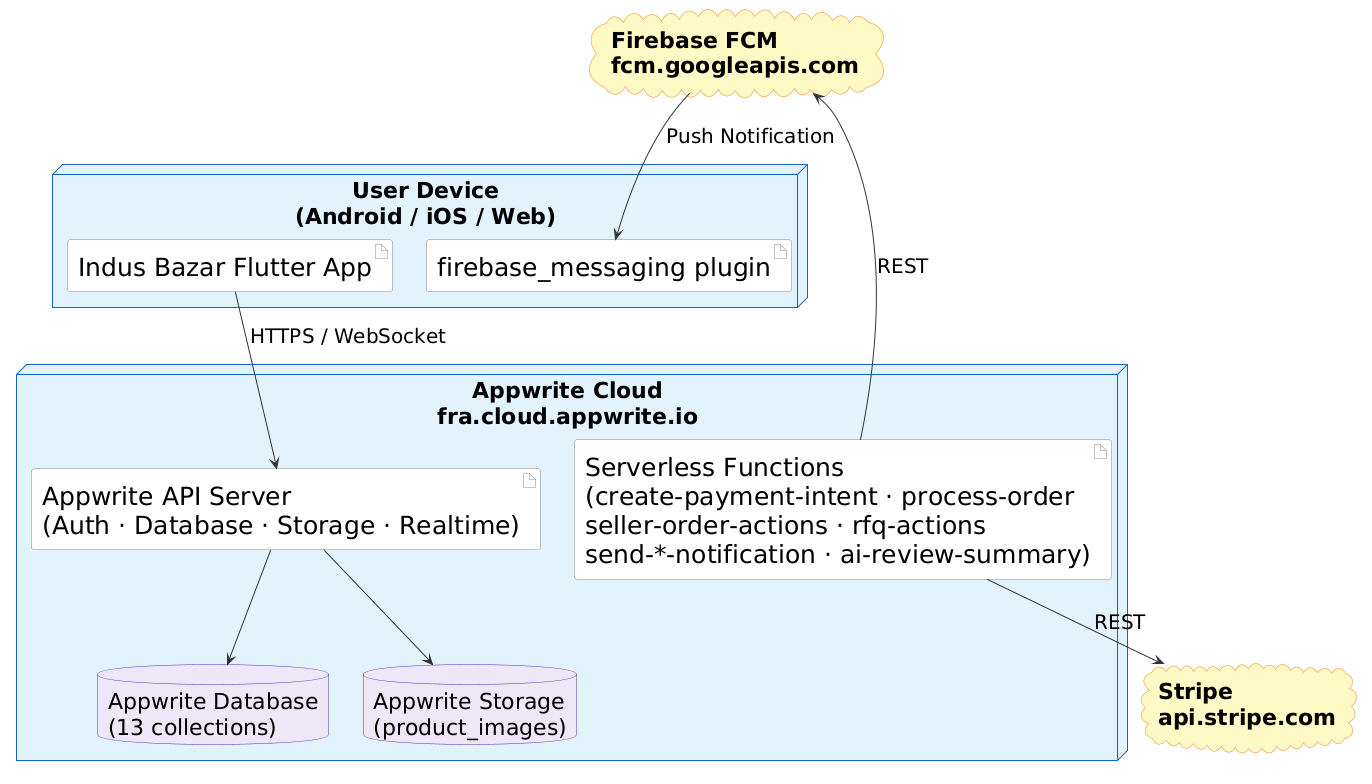
\includegraphics[width=1.0\textwidth]{figures/pictures project/deployment_diagram.png}
\caption{Deployment Diagram}
\label{fig:deployment_diagram}
\end{figure}

The deployment topology of Indus Bazar is depicted in the deployment diagram, as represented by Figure \ref{fig:deployment_diagram}. Flutter is executed as a native binary on the User's Device (Android or iOS) or a Progressive Web App in the browser. All backend requests are deployed to the Appwrite Cloud (located in the Frankfurt region at fra.cloud.appwrite.io) which contains internally the Appwrite API server, document database, file storage bucket, the Realtime subscription broker, and the serverless function runtime. The cloud functions call the Rest API of Stripe (api.stripe.com) to process payments and push notification delivery using Firebase Cloud Messaging (fcm.googleapis.com). The firebase\_messaging Flutter plug handles device-side notification handling by receiving the message sent by FCM.

\section{Sequence Diagrams}

The sequence diagrams in this section trace the interaction of the Flutter application, Appwrite services and external APIs to achieve each major feature of Indus Bazar. The diagrams show the appropriate actors, subsystems and system components, and provide a clear way of seeing the exact sequence of messages sent back and forth, the flow of data and the control logic used in the implementation of core functionalities within the platform. These charts emphasize both the synchronous and asynchronous communications, backend operations via Appwrite cloud functions, and secure connections with third-party services like Stripe to handle payments and Firebase Cloud Messaging to receive push notifications. The sequence diagrams offer an informative temporal perspective of how the system interacts with other systems, which verify the functional requirements and are useful in developing the system efficiently, debugging, testing, and scaling the Indus Bazar B2B marketplace in the future.

\clearpage
\subsection{Registration \& Login Sequence}

{\centering
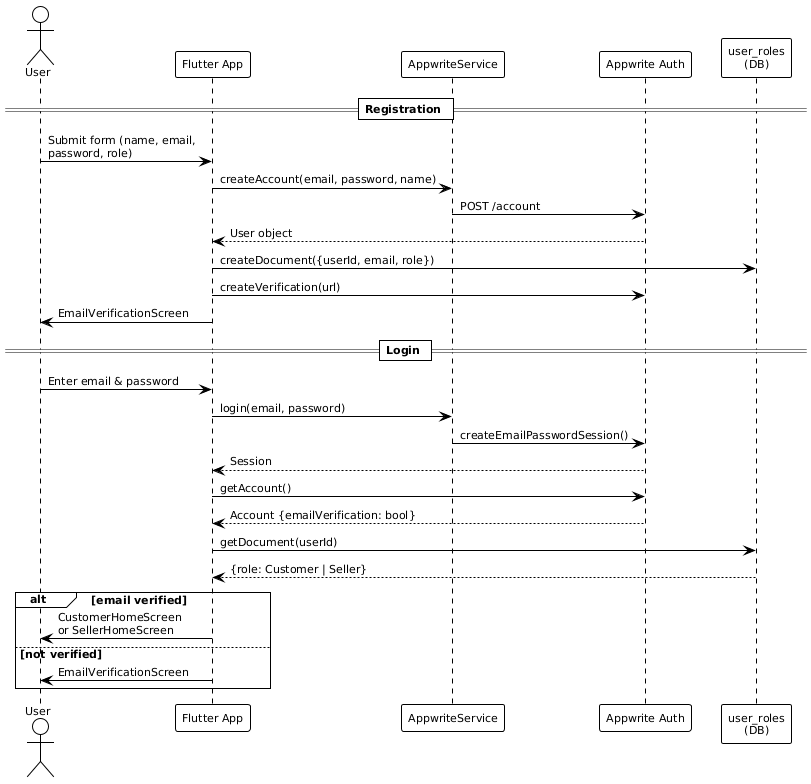
\includegraphics[width=\textwidth,height=0.75\textheight,keepaspectratio]{figures/pictures project/SEQUENCE1.png}\par
\captionof{figure}{Registration and Login Sequence Diagram}
\label{fig:login_sequence}\par}
\vspace{2em}

The sequence diagram of registration and login process \ref{fig:login_sequence} shows the two step onboarding process. In the course of the registration, the Flutter application invokes AppwriteService.createAccount, a call to the Appwrite Account API to create a new user. The selected role (Customer or Seller) is written to the collection of user roles in a follow up call, and an email verification message is sent. The user is then taken to the EmailVerificationScreen. At login, the app invokes AppwriteService.login(appwrite) that establishes an email-password session. Only when the validation is found, the AuthProvider gets the current account and role, verifies emailVerification status and redirects to the correct home screen (CustomerHomeScreen or SellerHomeScreen). Conflicts that occur during existing-session are managed in a transparent manner by catching the user\_session\_already\_exists error and reusing the valid session.

\subsection{Product Browsing \& Direct Purchase Sequence}

{\centering
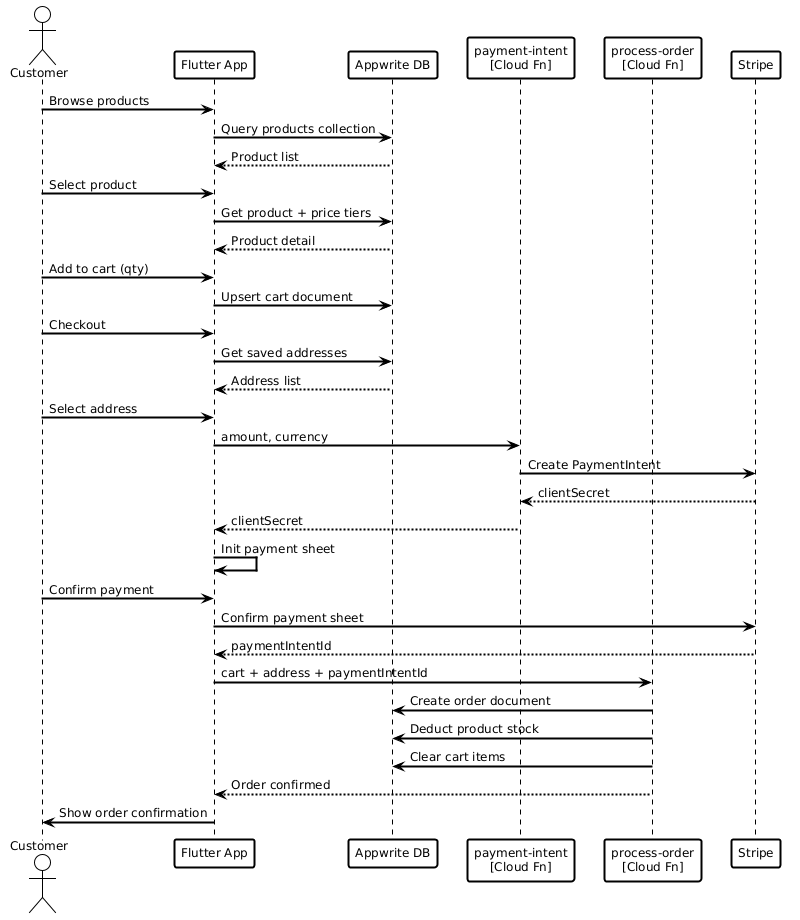
\includegraphics[width=\textwidth,height=0.75\textheight,keepaspectratio]{figures/pictures project/SEQUENCE2.png}\par
\captionof{figure}{Product Browsing and Direct Purchase Sequence Diagram}
\label{fig:product_browse_sequence}\par}
\vspace{2em}

The direct purchase sequence product browsing and direct purchase sequence \ref{fig:product_browse_sequence} encompasses the process of catalogue discovery to final payment. The customer clicks on ProductBrowseScreen, which calls upon ProductProvider to query the Appwrite products collection with optional category and search filters. When a product is selected, the ProductDetailScreen retrieves all the product information such as all price points and the seller profile and shows the tiered price structure. The customer enters the required amount to the cart; the CartProvider calculates the appropriate tier price and inserts a document into the cart collection. The customer chooses one of the saved addresses (or adds one to the addresses collection) at checkout, and PaymentProvider makes a create-payment-intent cloud call to StripeService, which returns a clientSecret. The Flutter Stripe payment sheet is loaded and shown; when it is confirmed Stripe returns a paymentIntentID, forwarded to the process-order cloud function. That atomically inserts the order document into the orders collection, removes stock off the product document and clears the cart items all under API-key authority of the server to pass through RLS.

\subsection{RFQ Creation \& Quote Acceptance Sequence}

{\centering
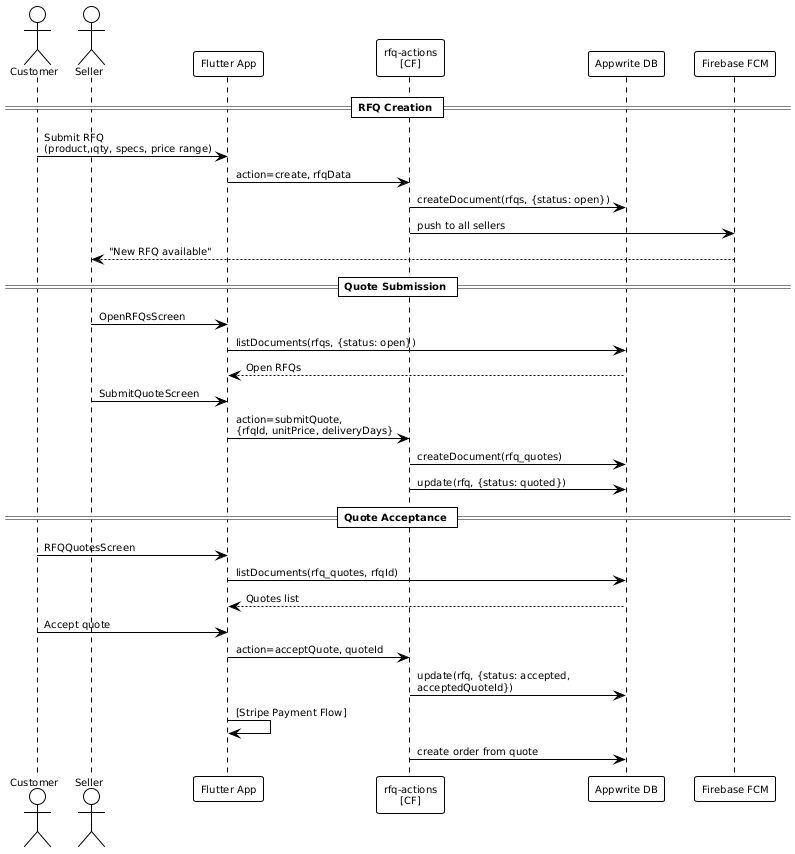
\includegraphics[width=\textwidth,height=0.75\textheight,keepaspectratio]{figures/pictures project/SEQUENCE3.png}\par
\captionof{figure}{RFQ Creation and Quote Acceptance Sequence Diagram}
\label{fig:rfq_sequence}\par}

The RFQ sequence diagram \ref{fig:rfq_sequence} follows the entire lifecycle of a Request for Quotation. The customer browses to CreateRFQScreen and sends a request with the name of products, category, quantity, city of delivery, deadline, specifications and optional target price range. The rfq-actions cloud function creates an RFQ document in the rfqs collection with status open and broadcasts a push notification via the send-rfq-notification function to all sellers. When an RFQ is made open, the sellers see it on OpenRFQsScreen, choose one of the relevant requests, and send the quote using SubmitQuoteScreen--the functionality stores the quote in rfq\_quotes and changes the status of the RFQ to quoted. RFQQuotesScreen: The customer evaluates all the quotes received and accepts one of them and goes to the payment flow through the same Stripe payment-sheet as with direct purchase. When payment is confirmed the process-order function produces the appropriate order and the RFQ status changes to accepted.

\subsection{Order Processing Sequence}

{\centering
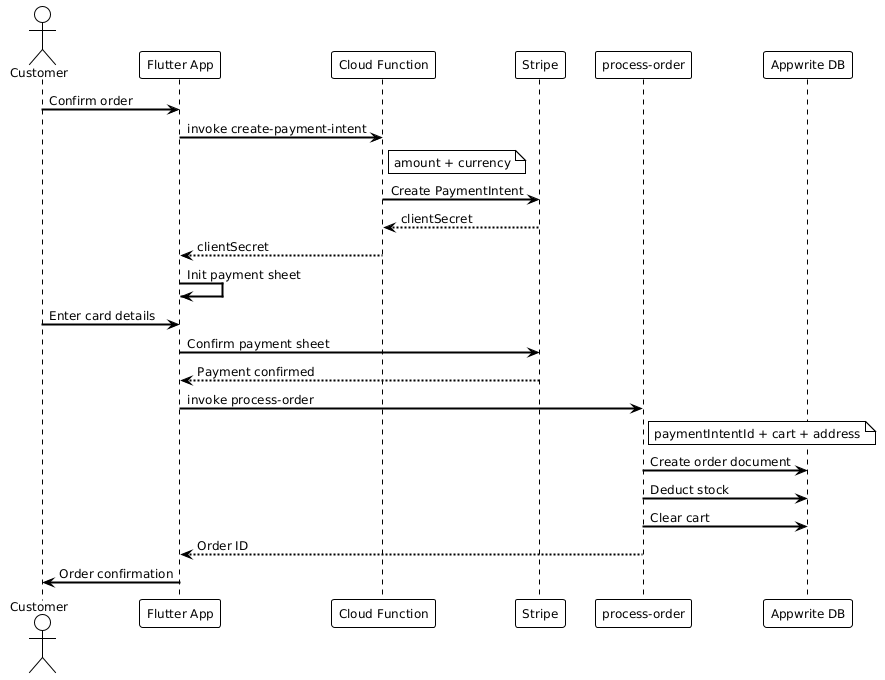
\includegraphics[width=\textwidth,height=0.75\textheight,keepaspectratio]{figures/pictures project/SEQUENCE4.png}\par
\captionof{figure}{Order Processing Sequence Diagram}
\label{fig:order_sequence}\par}

\vspace{1em}
The order processing sequence \ref{fig:order_sequence} shows the flow of order through its lifecycle after it has been created. When order document is present in the orders collection with the status pending, send-order-notification function sends an FCM push notification to the seller. The new order is displayed to the seller on the SellerOrdersScreen and can be viewed by the seller on SellerOrderDetailScreen (its contents, delivery address, contact with the customer) The seller actions (confirm, ship, deliver, cancel) are directed to the seller-order-actions cloud function that updates the order document status under API-key authority (bypassing the customer-only RLS on that document) and sends the corresponding send-order-notification call to ensure that the customer gets a live push notification. Status is followed by customer using the OrdersScreen.

\subsection{Real-Time Chat Sequence}

{\centering
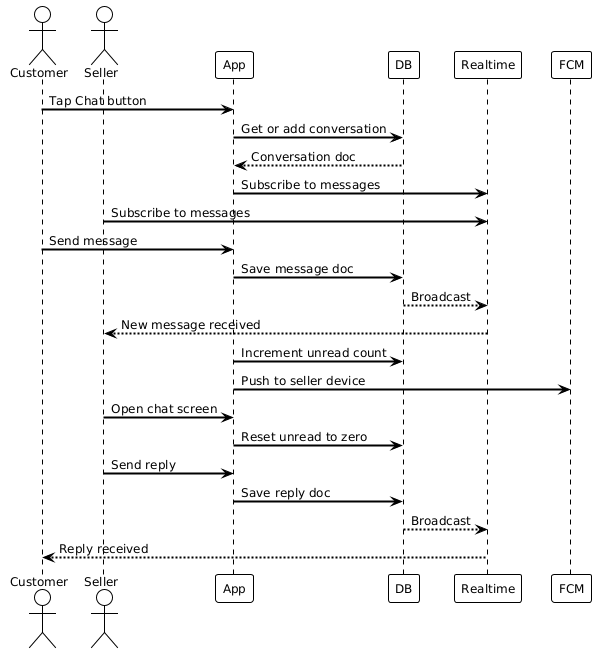
\includegraphics[width=\textwidth,height=0.75\textheight,keepaspectratio]{figures/pictures project/SEQUENCE5.png}\par
\captionof{figure}{Real-Time Chat Sequence Diagram}
\label{fig:chat_sequence}\par}

\vspace{1em}
The real-time chat sequence \ref{fig:chat_sequence} covers the establishment and operation of a product-scoped conversation between a customer and a seller. Upon the customer tapping the chat button on ProductDetailScreen, ChatService.getOrCreateConversation() searches the conversations collection to find an existent thread with key (customerId, sellerId, productId). In case none is available, a new conversation document is created with per-user Read and Update permissions. The ChatScreen is opened by both parties and subscribes to the Appwrite Realtime channel used to collect the messages with a conversationId filter. Messages sent are written to the messages collection and are immediately sent to all subscribers. When the send-chat-notification function is called every time to send a FCM notification to the recipient.

\subsection{Push Notification Delivery Sequence}

{\centering
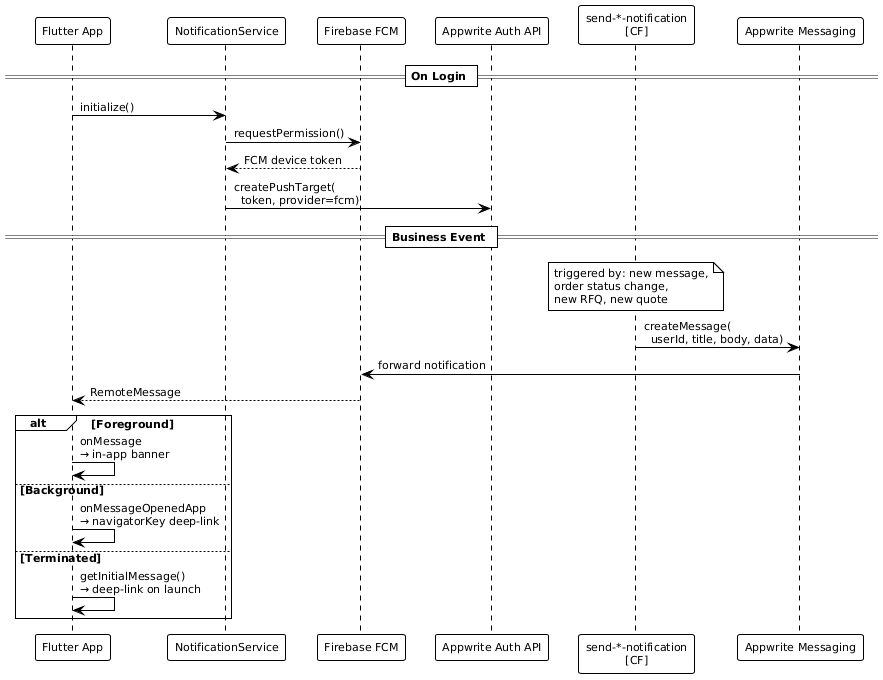
\includegraphics[width=\textwidth,height=0.75\textheight,keepaspectratio]{figures/pictures project/SEQUENCE6.png}\par
\captionof{figure}{Push Notification Delivery Sequence Diagram}
\label{fig:notification_sequence}\par}

\vspace{1em}
The notification delivery sequence \ref{fig:notification_sequence} shows the end to end flow of the event that triggers the notification, as well as the flow to the device of the recipient. Upon login, the Notificationservice makes a request to FCM permission, obtains the device FCM token and registers it as an Appwrite push target with the scope of the authenticated user. Upon a business event happening (new chat message, order status change, new RFQ, new quote), the call of the Appwrite Messaging API with the API key is made to generate a push message that will be sent to the relevant user registered FCM token. The message is sent to the Firebase Cloud messaging service, which sends it to the target device, through Appwrite. FirebaseMessaging is the notification that is processed by the firebase\_messaging plugin: when the app is in the foreground, it is FirebaseMessaging.onMessage is fired; when the app is in the background or terminated, onBackgroundMessage or getInitialMessage is called. On notification tap, the navigatorKey is used by \_handleNotificationTap (e.g., chat, order detail, RFQ list) to deep-link the user to the appropriate screen.

\section{Low Level Design}

Low Level Design (LLD) outlines data structures and entity relationships on which the Indus Bazar system will be based. All long-term data is stored in the NoSQL document collections in Appwrite; the schema below defines the values and relationships of each collection.

\subsection{UML Class Diagrams}
The Indus Bazar data model includes thirteen collections. The UML Class diagrams below illustrate the attributes of the entities and the referential associations to be kept using stored ID fields, which is a document-oriented database as Appwrite is.

\begin{figure}[H]
\centering
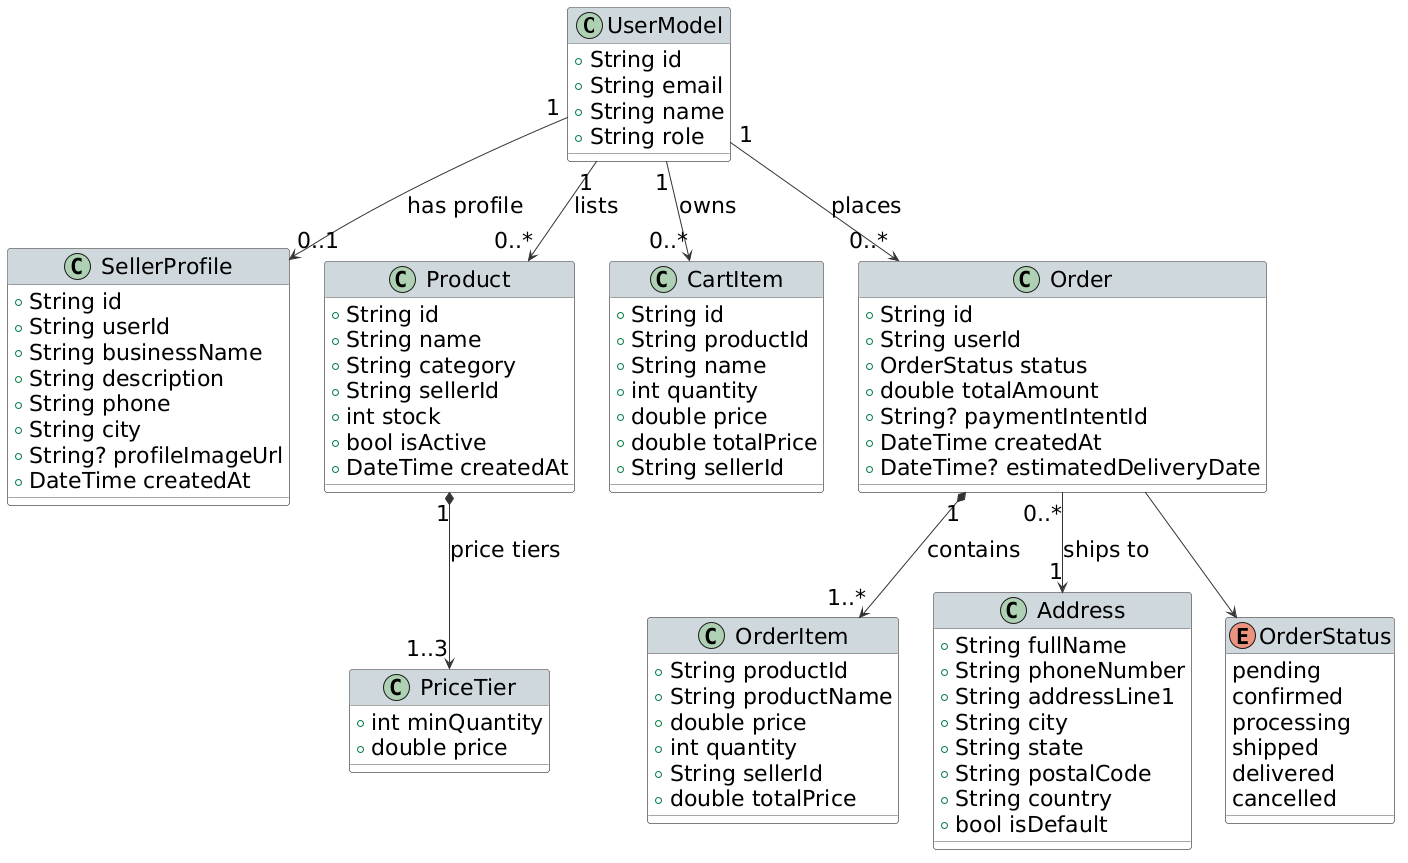
\includegraphics[width=0.95\textwidth]{figures/pictures project/UML_CLASS1.png}
\caption{Core Entity Relationship Diagram --- User, Product, Cart, Order, and Address Entities}
\label{fig:main_erd_schema}
\end{figure}

The backbone UML in Figure \ref{fig:main_erd_schema} deals with the transactional core of the marketplace. The \textbf{UserRoles} entity contains the following: userId, email, role (Customer / Seller), and fcmToken. The Product entity has name, description, category, sellerId, sellerName, stock, isActive, and up to three tiered price bands (tier1MinQty/tier1Price to tier3MinQty/tier3Price), with the imageUrls as a JSON-encoded array. The \textbf{CartItem} entity connects a user id to product id with a specified quantity. The \textbf{Order} object is a collection of customer information, a JSON array of items (each item is a productID, productName, price, amount, sellerID) total amount, status, paymentintentid and an embedded address. \textbf{The Address} entity holds street, city, province, postalCode and country and is referenced by both the order documents and the separate addresses collection of individual users.

\begin{figure}[H]
\centering
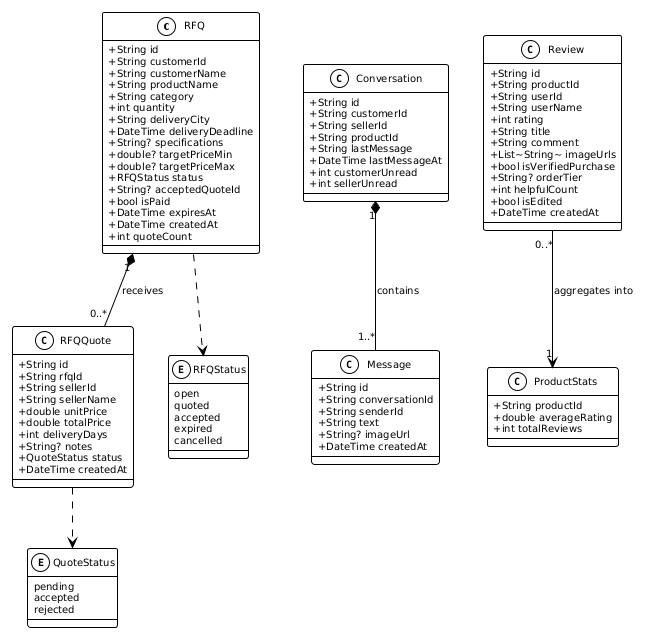
\includegraphics[width=0.95\textwidth]{figures/pictures project/UML_CLASS2.png}
\caption{Extended Entity Relationship Diagram --- RFQ, Chat, Review, and Seller Profile Entities}
\label{fig:extended_erd_schema}
\end{figure}

Figure \ref{fig:extended_erd_schema} is an extended UML that addresses the marketplace-specific and communication entities. The \textbf{customerId}, \textbf{category}, \textbf{productName}, \textbf{quantity} and \textbf{deliveryCity}, \textbf{deliveryDeadline}, \textbf{specifications}, optional \textbf{targetPriceMin/targetPriceMax}, \textbf{status (open / quoted / accepted / expired / cancelled)} and \textbf{expiresAt} are captured in the entity called the RFQ. Every \textbf{rfqQuote} is associated with a \textbf{sellerId} and \textbf{rfqId} having \textbf{unitPrice}, \textbf{totalPrice}, \textbf{leadTimeDays}, \textbf{notes} and a \textbf{status (pending / accepted / rejected)}. The \textbf{Conversation} entity has three-way key \textbf{customerId}, \textbf{sellerId}, and \textbf{productId}, \textbf{lastMessage}, \textbf{lastMessageAt}, \textbf{customerUnread}, and \textbf{sellerUnread}. Every \textbf{Message} is a member of a \textbf{conversationId} and contains \textbf{senderId}, \textbf{text}, \textbf{imageUrl} and \textbf{createdAt}. The \textbf{Review} entity associates a \textbf{userId} with a \textbf{productId} and storing \textbf{rating (1-5)}, \textbf{title}, \textbf{comment}, \textbf{JSON-encoded imageUrls}, \textbf{isVerifiedPurchase}, \textbf{helpfulCount} and \textbf{helpfulByUsers}. \textbf{ProductStats} is a pre-aggregated \textbf{averageRating}, \textbf{totalReviews}, and \textbf{rating-distribution counts}, per product. The \textbf{SellerProfile} table contains the attributes \textbf{userId}, \textbf{businessName}, \textbf{description}, \textbf{phone}, \textbf{address}, \textbf{city} (and \textbf{cityLower} as case-insensitive geosearch) and \textbf{profileImageUrl}.


\section{GUI Design}

The Indus Bazar mobile interface is structured on the concept of a role-adaptive experience: the application will have a different home screen and a flow of navigation depending on the role of the authenticated user (Customer or Seller). It is designed according to the Material Design 3 standards, with a custom AppTheme and looks into the usage of Google fonts, shimmer loading placeholders, cached\_network image as an efficient way to display images, and lottie animation as an empty and loading state. Every screen is created as HookConsumerWidgets, which rebuilds on Riverpod provider state changes.

\vspace{2em}

\begin{figure}[H]
\centering
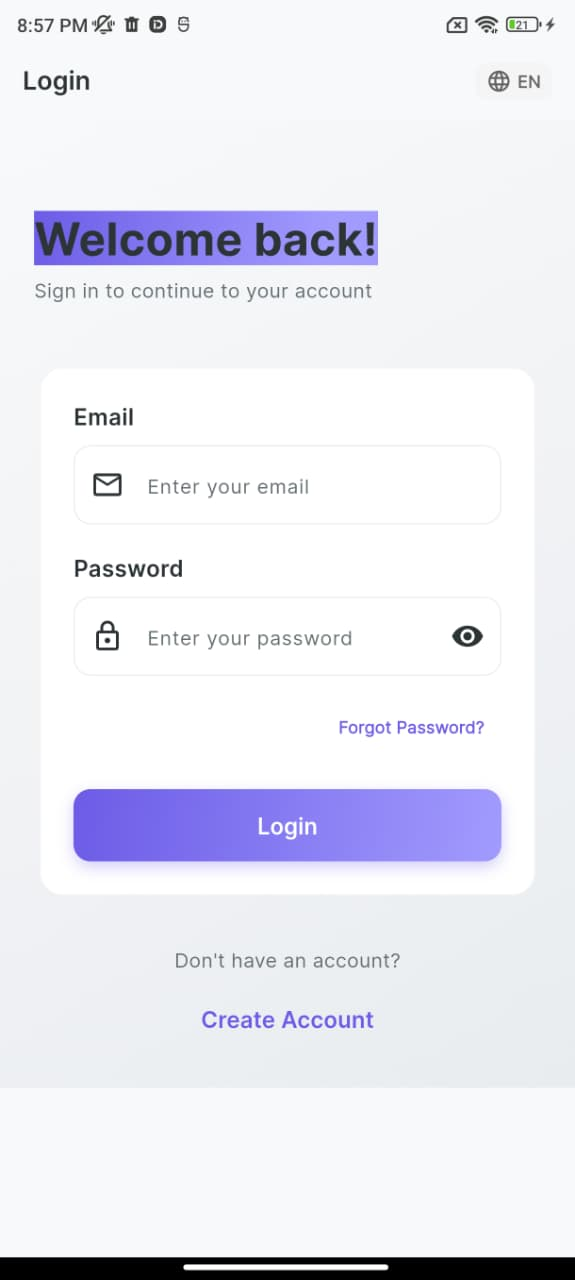
\includegraphics[width=0.4\textwidth]{figures/pictures project/frontend/login.jpeg}
\caption{Login Screen Interface}
\label{fig:login_screen}
\end{figure}

Figure \ref{fig:login_screen} shows the login interface of Indus Bazar. The screen offers a clear and bare bone of the registered user, and the input fields of email and password are assigned, a toggle of visibility of password is available, an option to forget password is present, and a large login button is presented on the screen. There is also a language switch in the upper right-hand corner where the user may switch language of the interface to proceed with the authentication. In terms of usability, the screen minimizes cognitive load by displaying minimal actions when signing in. The visual hierarchy established through the headline, form card and primary action button assist the user to learn the purpose of the page in a few seconds. The large distance between the input fields is also a good way to enhance the readability and touch response of the mobile devices. The design creates a very appropriate first-time and returning user experience since it does not have any distractions that would give the impression of a repetitive authentication pattern. Moreover, the form layout promotes validation and error messages in such a manner that they can be incorporated without disrupting the overall balance of the screen. Consequently, the login screen serves as a secure authentication point as well as the properly designed starting point of the role-based navigation of the application.


\begin{figure}[H]
\centering
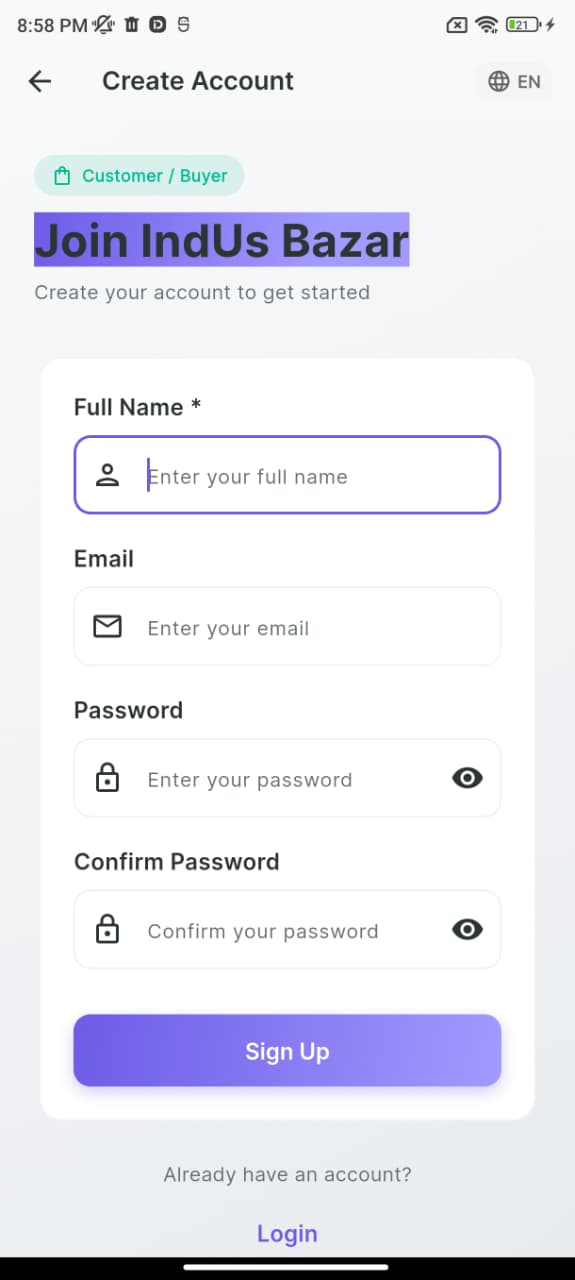
\includegraphics[width=0.4\textwidth]{figures/pictures project/frontend/signup.jpeg}
\caption{Registration Screen Interface}
\label{fig:signup_screen}
\end{figure}

Figure \ref{fig:signup_screen} presents the customer registration screen. The interface takes the required onboarding information such as full name, email address, password, password confirmation, and it has made it clear which role has been selected as Customer / Buyer. Its simple design enables less friction when creating an account and directs new users to the platform with the least friction. The shape will ensure that the onboarding process is explicit and linear so that users do not have to go through several steps before they complete the registration process. The role indicator is particularly essential in a two-role marketplace as it avoids confusion in creating customer and seller accounts. The visual consistency to the login screen also makes the users feel that the two screens are part of the same secure authentication process. The form is simple, with only one main sign-up button, which promotes form completion and maintains the model of interaction. This screen thus becomes significant in converting unidentified users into authenticated ones who can enjoy more of the market place. It also provides the first identity context that subsequently manages the role-based dashboard routing and permission-handling.

\begin{figure}[H]
\centering
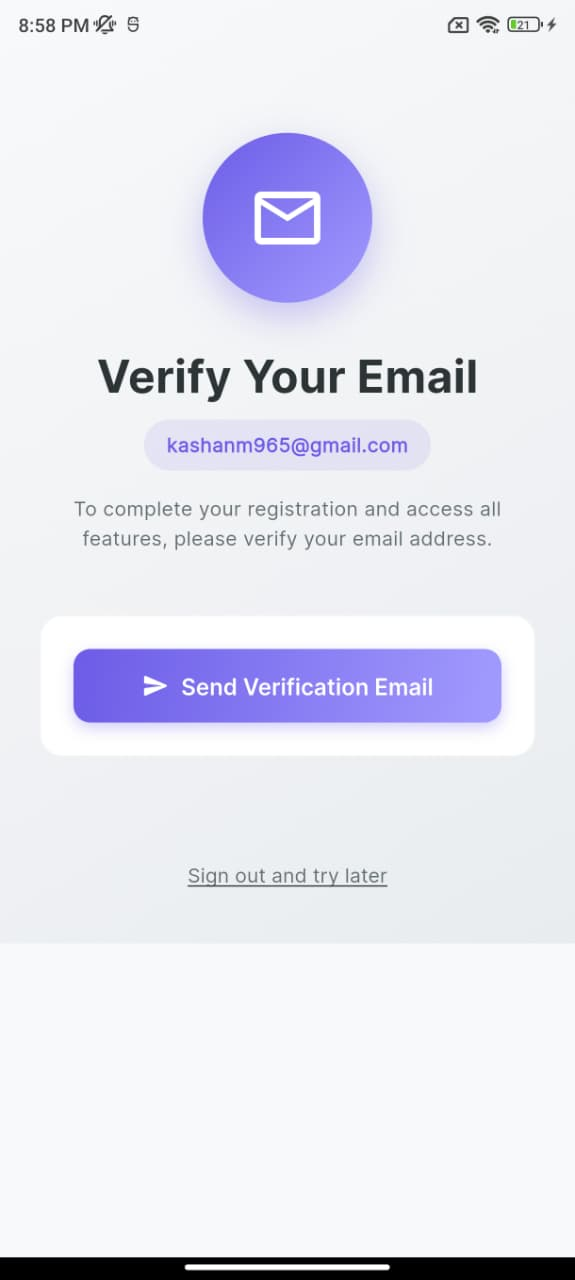
\includegraphics[width=0.4\textwidth]{figures/pictures project/frontend/email verification.jpeg}
\caption{Email Verification Screen Interface}
\label{fig:email_verification_screen}
\end{figure}

\clearpage

Figure \ref{fig:email_verification_screen} shows the email verification screen which appears after the registration. The screen notifies the user that they must activate the account to use the marketplace features and offers a specific action to resend the verification email in case it is necessary. This interface assists with the security need of the system that only a verified account can be given access to the main application. The use of the middle-ground composition and the targeted message makes it more than clear what the screen is all about and makes the user less likely to be confused post-account creation. The interface also informs the user that the request to verify his/her email address has been sent by showing him/her the email address and also reminds him/her in case of typing errors. Reliability is also significant with resend action, when mail delivery can be delayed, or lost messages. The signature out and resume option also conforms to the real world user behaviour, by permitting temporary suspension without disrupting the flow. Security wise, this screen enhances the degree of trust because it physically implements account validation as opposed to unverified access. Generally, it serves as a gate between registration and the actual system use.

\begin{figure}[H]
\centering
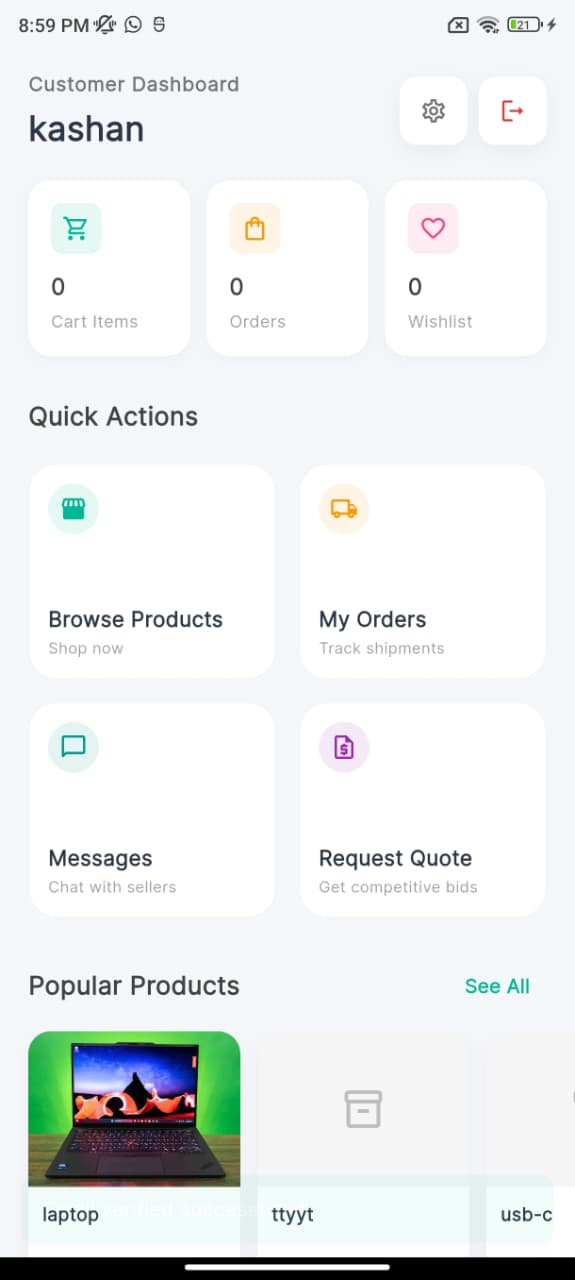
\includegraphics[width=0.4\textwidth]{figures/pictures project/frontend/customer dashboard.jpeg}
\caption{Customer Home Screen Interface}
\label{fig:customer_home}
\end{figure}

\clearpage
The customer home dashboard as depicted in Figure \ref{fig:customer_home} serves as the main area of navigation when the customer is already logged in. It provides an overview of important user metrics (cart items, orders, and wishlist items), and has quick-action cards to browse the products, track the orders, open the messages and create RFQs. There is also a popular products section to bring out featured items and stimulate product discovery. This screen has been created to reduce the effort of navigation because the most common customer activities are put together. The metric cards also give the client a real-time feedback on what is going on in the marketplace and make the user know their position within the application. Quick-action tiles are visual shortcuts that minimise the amount of steps that have to be followed in between to get to the popular workflows. The featured or popular products are also added to the dashboard turning the dashboard into a commercial discovery-based surface rather than the functional one. This plays a critical role in a B2B market where decisions to buy are frequently influenced by repeated shopping and comparison of products. The dashboard thus contributes not only to efficiency in carrying out the tasks, but also to engagement with the product, thus, being a vital aspect of the customer experience. The role-adaptive design philosophy can be seen in its design as well since it reveals functions that are pertinent to buyers.

\begin{figure}[H]
\centering
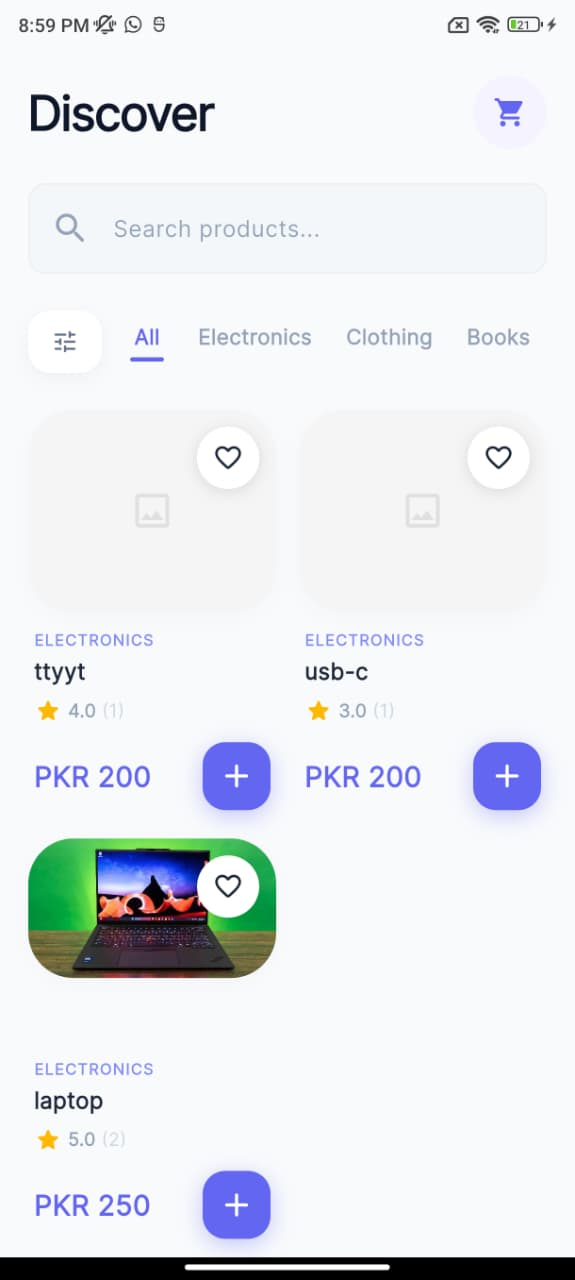
\includegraphics[width=0.3\textwidth]{figures/pictures project/frontend/discover.jpeg}
\caption{Product Browse Screen Interface}
\label{fig:product_browse_screen}
\end{figure}

The product browsing screen Figure \ref{fig:product_browse_screen} is a customer-facing screen where customers can browse through the available products within the catalogue. The interface is a combination of a search box, filtering categories, shortcuts to the wishlist, product ratings, price, and the quick add-to-cart buttons in a scrollable design. This design enables the effective product discovery as users can narrow results and perform actions on products right in the listing view. The navigation is designed to be scanned quickly and allow the user to browse through multiple products without having to open each product separately. The tabs of categories assist in grouping the catalogue in familiar commercial groupings, which is particularly helpful as the marketplace expands. The search query also facilitates the specific product search when the user is aware of what they want to buy. Visual product cards strike a balance between commercial data like price and rating and actionable controls, like the add-to-cart button. This minimizes the purchasing process and enables the customer to speed up his/her discovery to choice. The page is also conducive to exploratory behaviour with several choices in a small yet readable format. Consequently, it serves as the main catalogue interface to provide convenient browsing and make purchases in advance.

\begin{figure}[H]
\centering
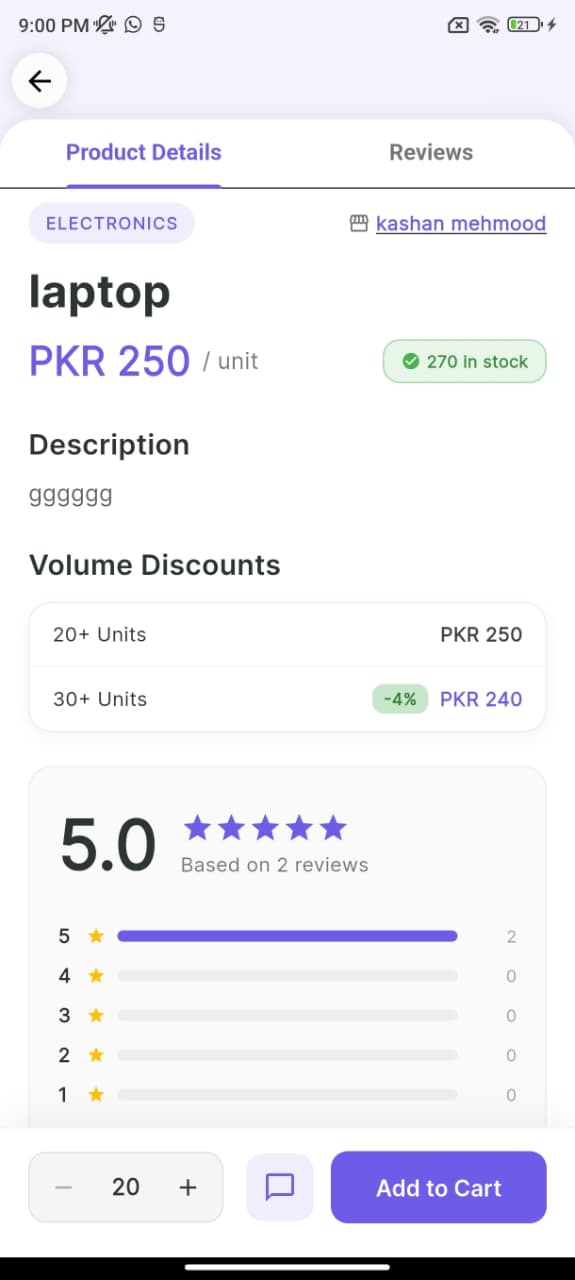
\includegraphics[width=0.4\textwidth]{figures/pictures project/frontend/product description.jpeg}
\caption{Product Detail Screen with Tiered Pricing Interface}
\label{fig:product_detail_screen}
\end{figure}

The product detail screen is shown in figure \ref{fig:product_detail_screen} where the customer has the opportunity to view all the information about the item before buying. The interface displays the category and seller of the product, stock, description, quantity selection, customer review summary and the tiered pricing table which increases or decreases the value based on the volume of bulk purchases. It also gives direct actions to start a chat with the seller and add the number of items chosen to the cart. This is a crucial screen especially in a B2B situation since it is in such a case that buyers require more commercial information before they commit to an order. The availability symbol and the seller identification assists in creating trust and buying confidence. One of the fundamental marketplace features is relayed through the volume discount section which displays the price change with the increase in the quantity of an order. The summary of the reviews also helps make a decision, bringing out the feedback of the collective customers on the same screen. The quantity and persistent action buttons ensure that the purchase process is as near to the product description as possible, without having to navigate further. This screen is the prime point of conversion in the direct-purchase journey by integrating evaluation, communication, and preparation of transactions in a single display. It is thus one of the most densely functional and business important interfaces in the system.

\begin{figure}[H]
\centering
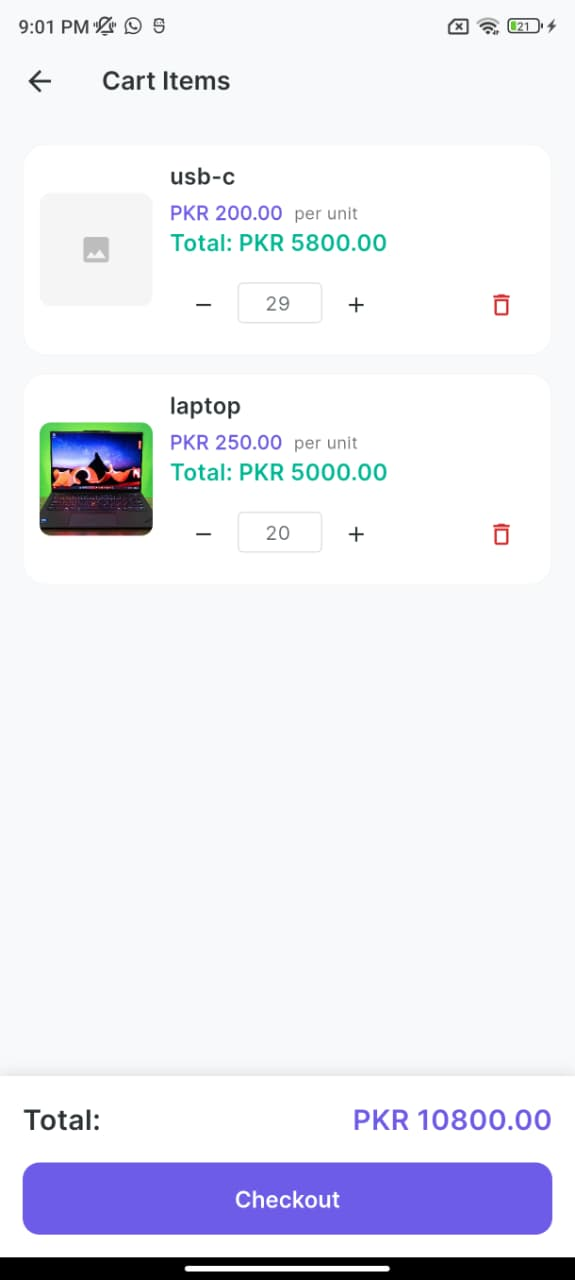
\includegraphics[width=0.3\textwidth]{figures/pictures project/frontend/cart items.jpeg}
\caption{Cart Screen Interface}
\label{fig:cart_screen}
\end{figure}

The cart screen in Figure \ref{fig:cart_screen} is used to gather the selected items prior to checkout. The interface displays all items in the products list their unit price, quantity adjustments, subtotal and remove feature and a running total displayed at the bottom of the screen. Such a design allows the customers to easily alter the quantity of orders and analyze the financial consequences of bulk orders prior to ordering them. The cart is a transient holding space that assists the customers in narrowing down on the decisions they are likely to make in making their purchase decisions prior to making any payments. The controls of quantity increment and decrement are used to facilitate real-time adaptation of order size which is particularly applicable when tiered pricing affects the overall prices. Table of per-item totals and the overall total enhance financial transparency and minimize uncertainty in the process of buying. The capability to delete items in the cart assists the user to have control over what they would like to order. Since the cart can group several products into a single list to be reviewed, it also facilitates the buying patterns of multi-item, which are typical of wholesale. The checkout button is placed as the next most important button and it allows one to be sure that the user will proceed to finalising the order. In general, this screen combines choice of products and formality processing of order in an effective manner.

\begin{figure}[H]
\centering
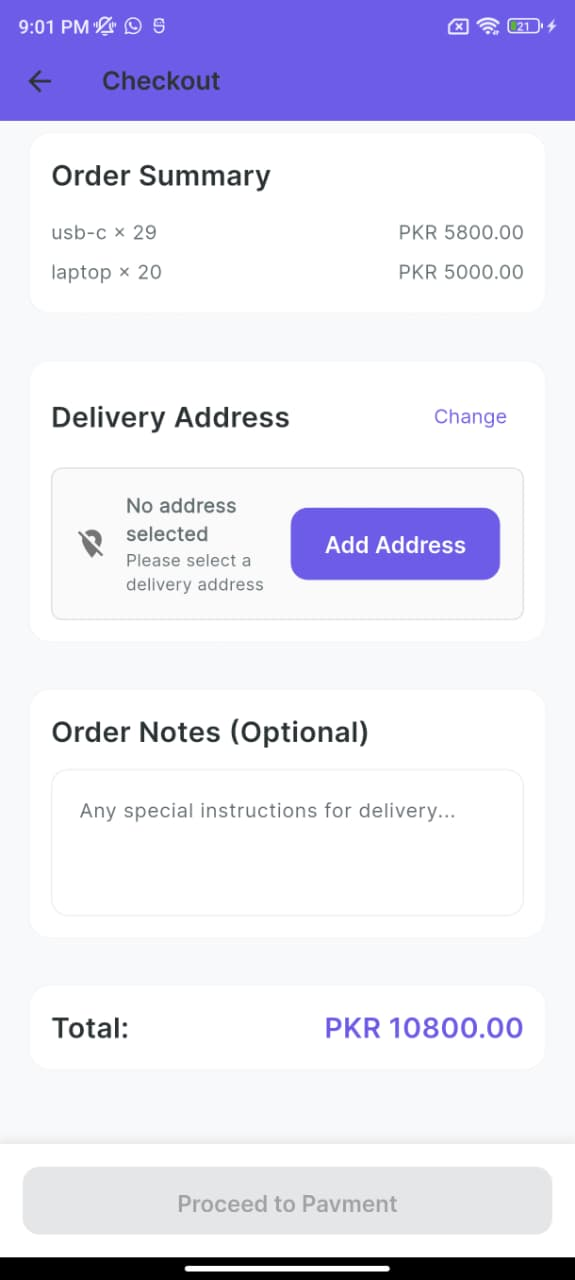
\includegraphics[width=0.4\textwidth]{figures/pictures project/frontend/order summary.jpeg}
\caption{Checkout and Payment Screen Interface}
\label{fig:checkout_screen}
\end{figure}

Figure \ref{fig:checkout_screen} shows the checkout screen that is used to complete an order. It summarises the chosen products, gives the user an opportunity to select or add an address in which to deliver the goods, gives them room to add optional delivery notes, and shows the amount they should pay. The screen serves as the last inspection point prior to the customer being taken through the safe payment channel. Practically, this interface would gather all the vital details of the order that have to be verified prior to the initiation of payment. The delivery address section plays a crucial part in particular since B2B transactions tend to require proper logistics information and destination management. Special instructions, optional notes allow flexibility, and could involve packaging, handling, or contact options. The segregation of order summary, address selection and note generates a systematic flow that minimizes chances of information omission. The placement of the total amount also helps to instill cost consciousness prior to payment verification. It is thus a usability checkpoint, as well as a data-validation step that will help in maintaining order accuracy. It is at the core of converting a shopping cart into a purchase request.

\begin{figure}[H]
\centering
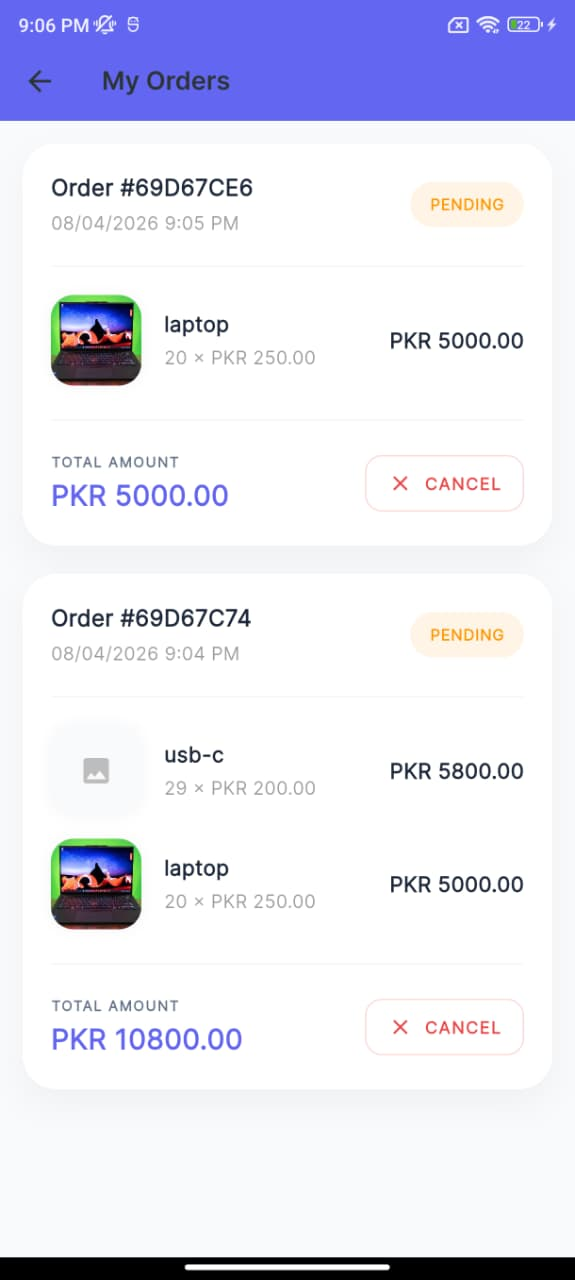
\includegraphics[width=0.4\textwidth]{figures/pictures project/frontend/my orders.jpeg}
\caption{Customer Orders Screen Interface}
\label{fig:orders_screen}
\end{figure}

The customer orders screen is shown in Figure \ref{fig:orders_screen} where the customer can view orders that have been placed in the past. The order cards show the order identifier, time, goods included, price, and processing status, and have the option to cancel orders (where possible). This screen enables the customers to have a clear picture of the history of purchase and the progress of their orders. The interface will also enhance transparency following payment with transaction records remaining transparent and easy to understand. The identifiers of order and timestamps assist users in distinguishing between several purchases and aid in the further reference in communication or dispute resolution. Status labels give a simple impression of the current stage of each order in the fulfilment lifecycle, pending confirmation to delivery. The item previews are also included to make the users remember the contents of every order without necessarily viewing the more detailed screens. This comes in handy especially in repeat-purchase environment where a customer might have a number of overlapping transactions. Canceling orders (where possible) provides the consumer with an added perceptions of control and flexibility. In sum, the orders screen assists in instilling confidence in the customers after purchase and continued management of the relationship between the customer and seller.

\begin{figure}[H]
\centering
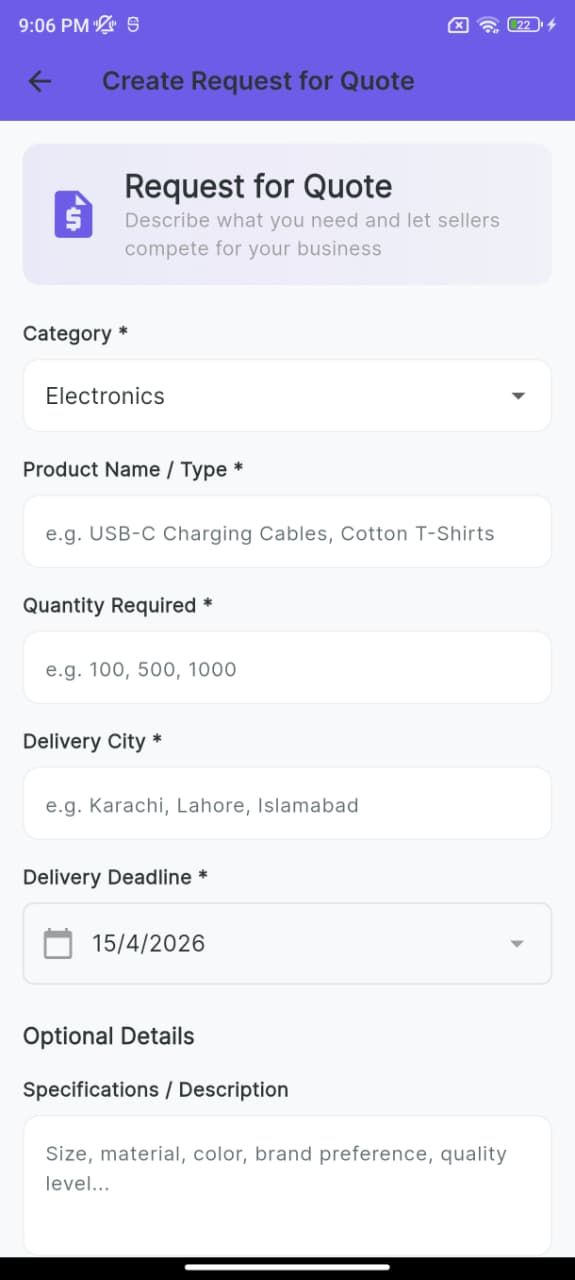
\includegraphics[width=0.4\textwidth]{figures/pictures project/frontend/request for qouta.jpeg}
\caption{Create RFQ Screen Interface}
\label{fig:create_rfq_screen}
\end{figure}

The creation form of quotation-based procurement is the RFQ creation form as shown in figure \ref{fig:create_rfq_screen}. The interface records the category, type of products, quantity needed, city of delivery, deadline and optional specifications in order to ensure that the customers indicate bulk or tailor-made purchasing requirements in a formal format. The design allows sellers to provide specific and competitive quotations. The RFQ workflow stands out as a differentiator of the marketplace since it goes beyond the fixed-price catalogue buying. The structure of the request of the customer in the form of specific fields guarantees the sellers that they will have sufficient information to make realistic offers. These are especially the delivery deadline and the destination in the context of commercial negotiations since they affect the cost, the feasibility and the anticipated lead time. The optional description fields also allow the customer to have some flexibility in describing what they want in quality, materials, or other desired attributes that were not easily available in standard product listing. The interface thus accommodates multi-faceted procurement situations that are prevalent in B2B trade. Its data format is organized and enhances the quality of data as well as the comparability of responses among sellers. This screen is efficient in converting customer demand into a formal marketplace opportunity that could be analyzed and responded to by a number of sellers.


\begin{figure}[H]
\centering
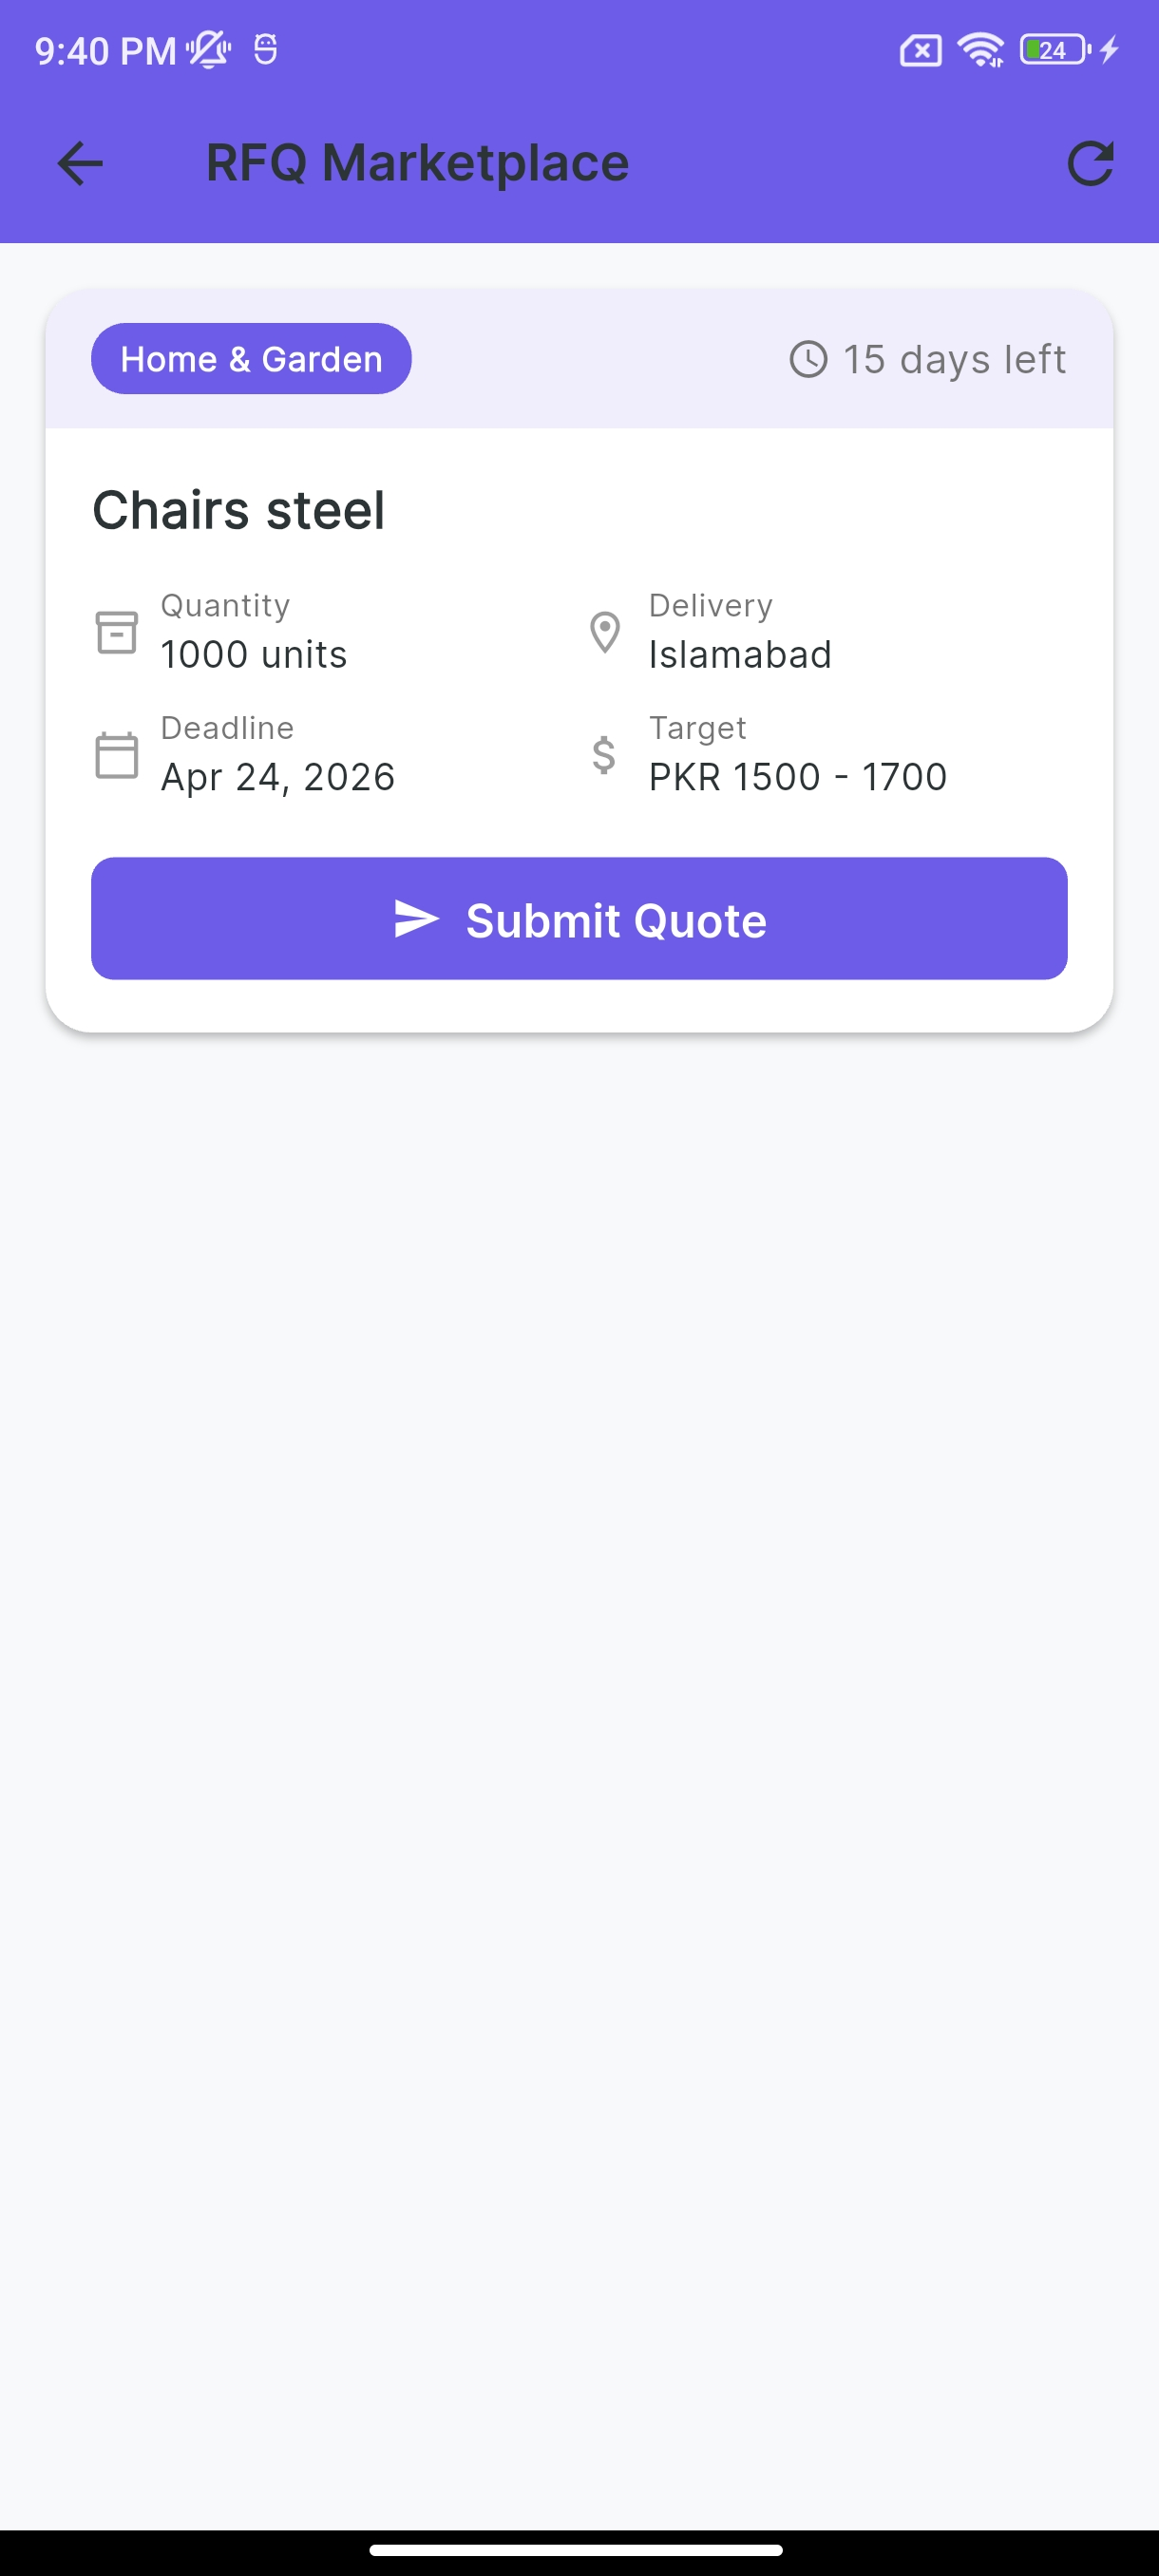
\includegraphics[width=0.4\textwidth]{figures/pictures project/sellerside/rfq market place.jpeg}
\caption{Open RFQ Marketplace Screen Interface (Seller View)}
\label{fig:open_rfqs_screen}
\end{figure}

Figure \ref{fig:open-rfqs-screen} shows the seller-side RFQ marketplace. The RFQ cards contain an overview of the request type, quantity, delivery address, due date and the approximate budget limit, and a direct quote-submission action. The interface enables sellers to find business opportunities they are interested in by aggregating open requests into a single marketplace. This screen will serve as a competitive demand board on which sellers will be able to scan on the open procurement requests and determine which business opportunities can be used in accordance to their inventory and business objectives. The card layout is summarised allowing quick comparison of various RFQs without having to navigate to different pages. Attributes that are of commercial interest like deadline and target budget assist sellers to prioritize the requests that have likelihood of turning into profitable deals. The direct submission cutoff also reduces the response cycle and promotes the participation of sellers in time. Such responsiveness is essential in a multi-seller marketplace to have an ecosystem of active quotations. The screen thus facilitates the opportunity discovery as well as transactional efficiency. It also shows how the platform goes beyond the traditional browsing by providing request-based commerce.

\begin{figure}[H]
\centering
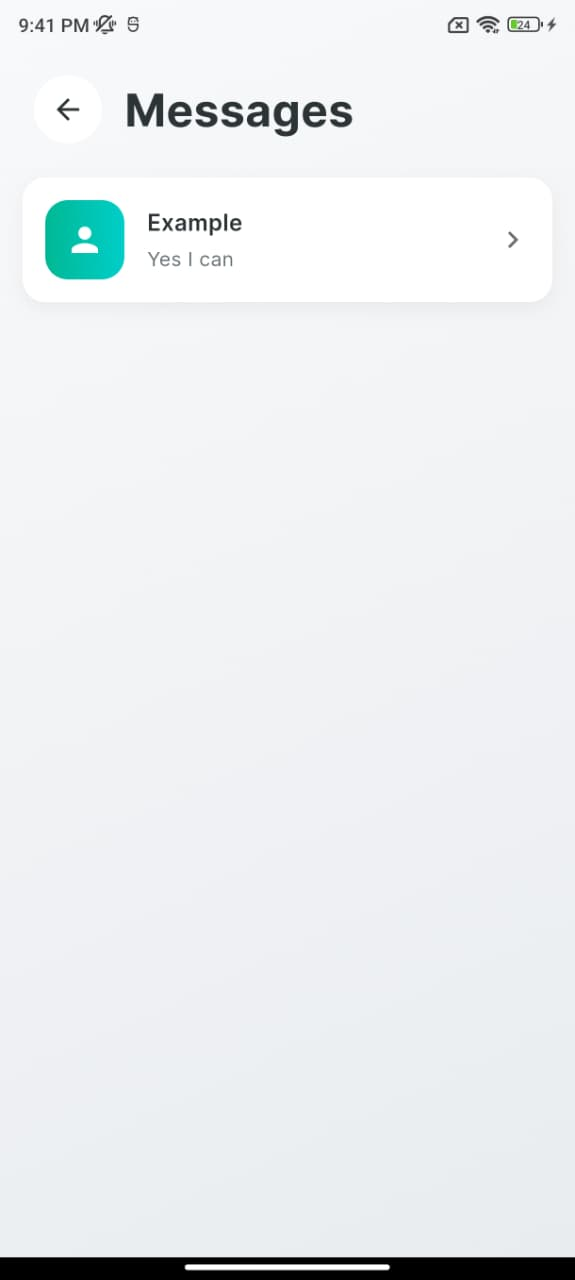
\includegraphics[width=0.4\textwidth]{figures/pictures project/sellerside/messages.jpeg}
\caption{Real-Time Chat Screen Interface}
\label{fig:chat_screen}
\end{figure}

Figure \ref{fig:chat_screen} is the messaging interface that is used to communicate between customers and sellers. The conversations are presented in a straightforward list format with the identity of the participants and the last message preview, and users can easily access current conversations. This screen aids the real-time interactive nature of the platform in clarifying products, orders and RFQ details. The communication is a necessity in the B2B trade, where the buyer and supplier frequently need to discuss quantities, verify specifications, or clarify the questions of fulfilment. The list-based form provides the user with a brief idea of the conversations taking place and allows them to easily locate the latest interaction. The preview of the latest message will enhance message-triage as the user will be able to gauge the relevance of a conversation even before opening it. The minimal design also makes the interaction lean and fits well in the common usage on mobile phones. Messaging imparts as a part and parcel of the marketplace; therefore, users do not have to switch to alternative means of communication. This reinforces a continuity between browsing, placing orders, RFQ management and post sales assistance. Consequently, the chat interface is a key to the responsive commercial coordination of both user roles.
\begin{figure}[H]
\centering
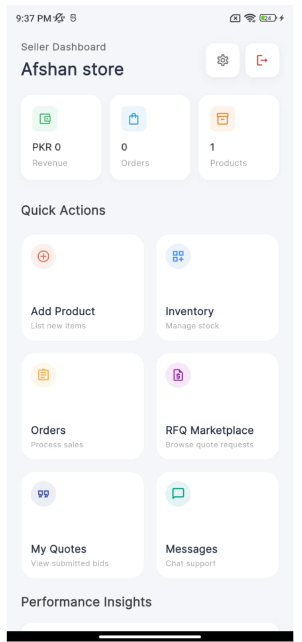
\includegraphics[width=0.4\textwidth]{figures/pictures project/sellerside/seller store.png}
\caption{Seller Home Screen Interface}
\label{fig:seller_home_screen}
\end{figure}

Figure \ref{fig:seller_home_screen} depicts the seller dashboard which is the key control panel of operations on the supplier side. It shows summary data like revenue, order count, products count, and offers fast actions to add products, inventory management, orders, RFQ review, and message review. This job-specific dashboard assists sellers to operate the activity of the marketplace at one point of entry. Operationally, the dashboard simplifies the process of working with sellers as it consolidates the key business functions on a single overview page. The summary cards enable sellers to quickly check their current performance without having to open numerous management screens. Quick-action tiles reduce the time taken in navigation and simplify repetitive processes, like updating inventory or reviewing orders. It is especially useful in a marketplace situation where sellers might be required to act fast in regard to the orders and quotation requests received. The dashboard also indicates the professional identity of the seller account, as the focus on the information regarding revenues and fulfilment is prioritised over consumer-centric browsing metrics. Its design thus favors both the operational consciousness and quick response. In general, it is the primary working environment of participation in a marketplace on the seller side.


\begin{figure}[H]
\centering
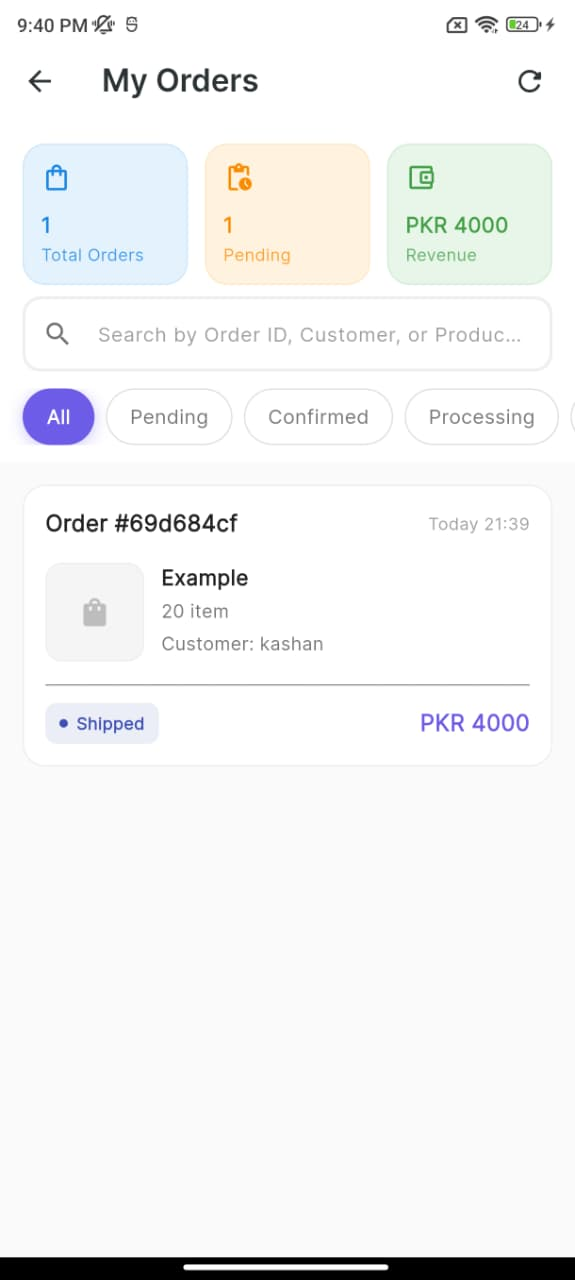
\includegraphics[width=0.4\textwidth]{figures/pictures project/sellerside/my orders.jpeg}
\caption{Seller Orders Management Screen Interface}
\label{fig:seller_orders_screen}
\end{figure}

The seller orders management screen is shown in figure \ref{fig:seller_orders_screen}. The interface provides overview of operating statistics, allows search and status-based filtering, and displays customer orders and item details, buyer details, order status and order value. It is created to assist sellers in monitoring progress in fulfilment and it also allows them to take orders effectively. The screen is customized to fulfilment management whereby sellers must track the flow of transactions and react based on the status of each order. Search and filter controls enhance scalability, because sellers can find particular orders in a short time, despite the growing volume of transactions. The presence of customer identity and item information in every order card facilitates quick decision-making in operations without having to change the pages all the time. Status visibility is particularly crucial since duties of the sellers vary with changes in the state of orders between pending and confirmed, shipped, and delivered. The situational awareness is also enhanced by the operational summary at the top of the screen that sums up important indicators related to orders. This interface thus integrates monitoring, filtering and preparation of actions in one management space. It is at the core of ensuring stable quality and punctuality in seller service.


\begin{figure}[H]
\centering
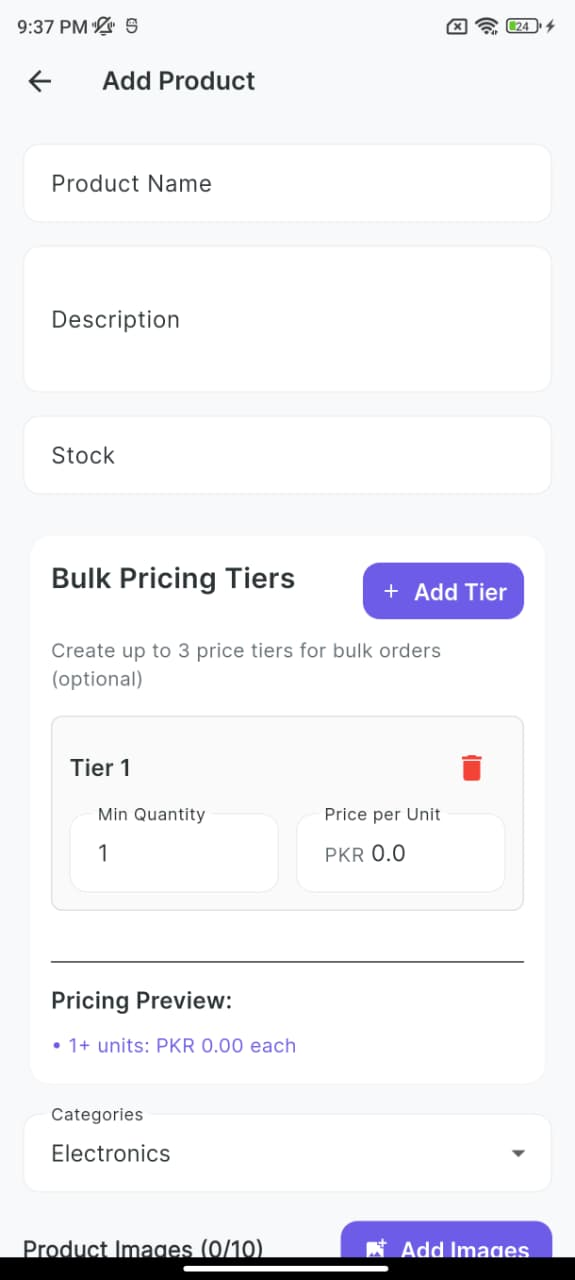
\includegraphics[width=0.4\textwidth]{figures/pictures project/sellerside/add products.jpeg}
\caption{Add Product Screen Interface (Seller)}
\label{fig:add_product_screen}
\end{figure}

The seller product creation interface can be seen in Figure \ref{fig:add_product_screen}. The form also has the product name, description, stock level, category, images and bulk pricing levels which enable the sellers to establish the normal pricing rules and volume-based pricing rules. This screen is crucial in sustaining a catalogue which is specific to wholesale and B2B buying behaviour. It is a form created to encompass a descriptive and a commercial part of a product within a single workflow. Fields like stock quantity and category will make sure that the products are displayed in the same way, and buyers can be able to find them correctly. This feature of the marketplace allowing the introduction of bulk pricing levels directly into the same interface emphasizes the fact that the marketplace supports the idea of commercial negotiations based on quantity. The ability to upload pictures also enhances the presentation of the products because the sellers can communicate the visual quality and the look of the products. The interface reduces the amount of effort needed to publish and manage inventory by putting all these features in a single screen. This plays a role in the involvement of sellers, as simple product creation will motivate a more abundant and lively marketplace catalogue. Effectively, the add-product screen fulfils the role of a seller as a supplier in the digital marketplace.

\begin{figure}[H]
\centering
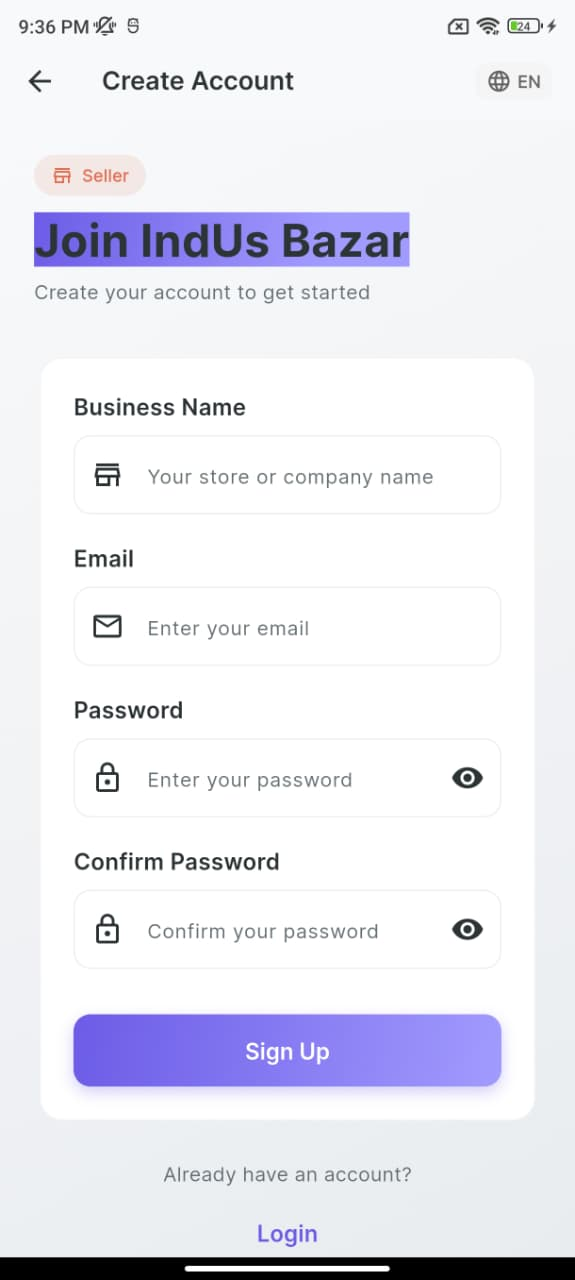
\includegraphics[width=0.4\textwidth]{figures/pictures project/sellerside/create account for seller.jpeg}
\caption{Seller Registration Screen Interface}
\label{fig:seller_profile_screen}
\end{figure}

The seller registration screen is depicted in figure \ref{fig:seller_profile_screen}. The interface gathers business name, email address, password and password confirmation with a clear indication that the account is a seller account. This role-specific onboarding perspective guarantees that the suppliers are introduced into the market by a special registration process. This interface, compared to the conventional customer registration, focuses more on business identity as opposed to personal identity, which is the nature of seller participation. The explicit seller label makes it less ambiguous and assists in aligning the expectations of users at the time of creating an account. It should be consistent with the overall authentication design so as to maintain familiarity yet make the supplier role visually distinct. This role division is significant in that, seller accounts subsequently access specialised dashboards and management tools that buyers do not have access to. The form is clean, which means that it also contributes to fast completion and ease in verifying the needed information. The screen helps to classify accounts correctly and control access by taking suppliers through a different onboarding route. It is thus a significant initial phase of the seller lifecycle in the platform.

\begin{figure}[H]
\centering
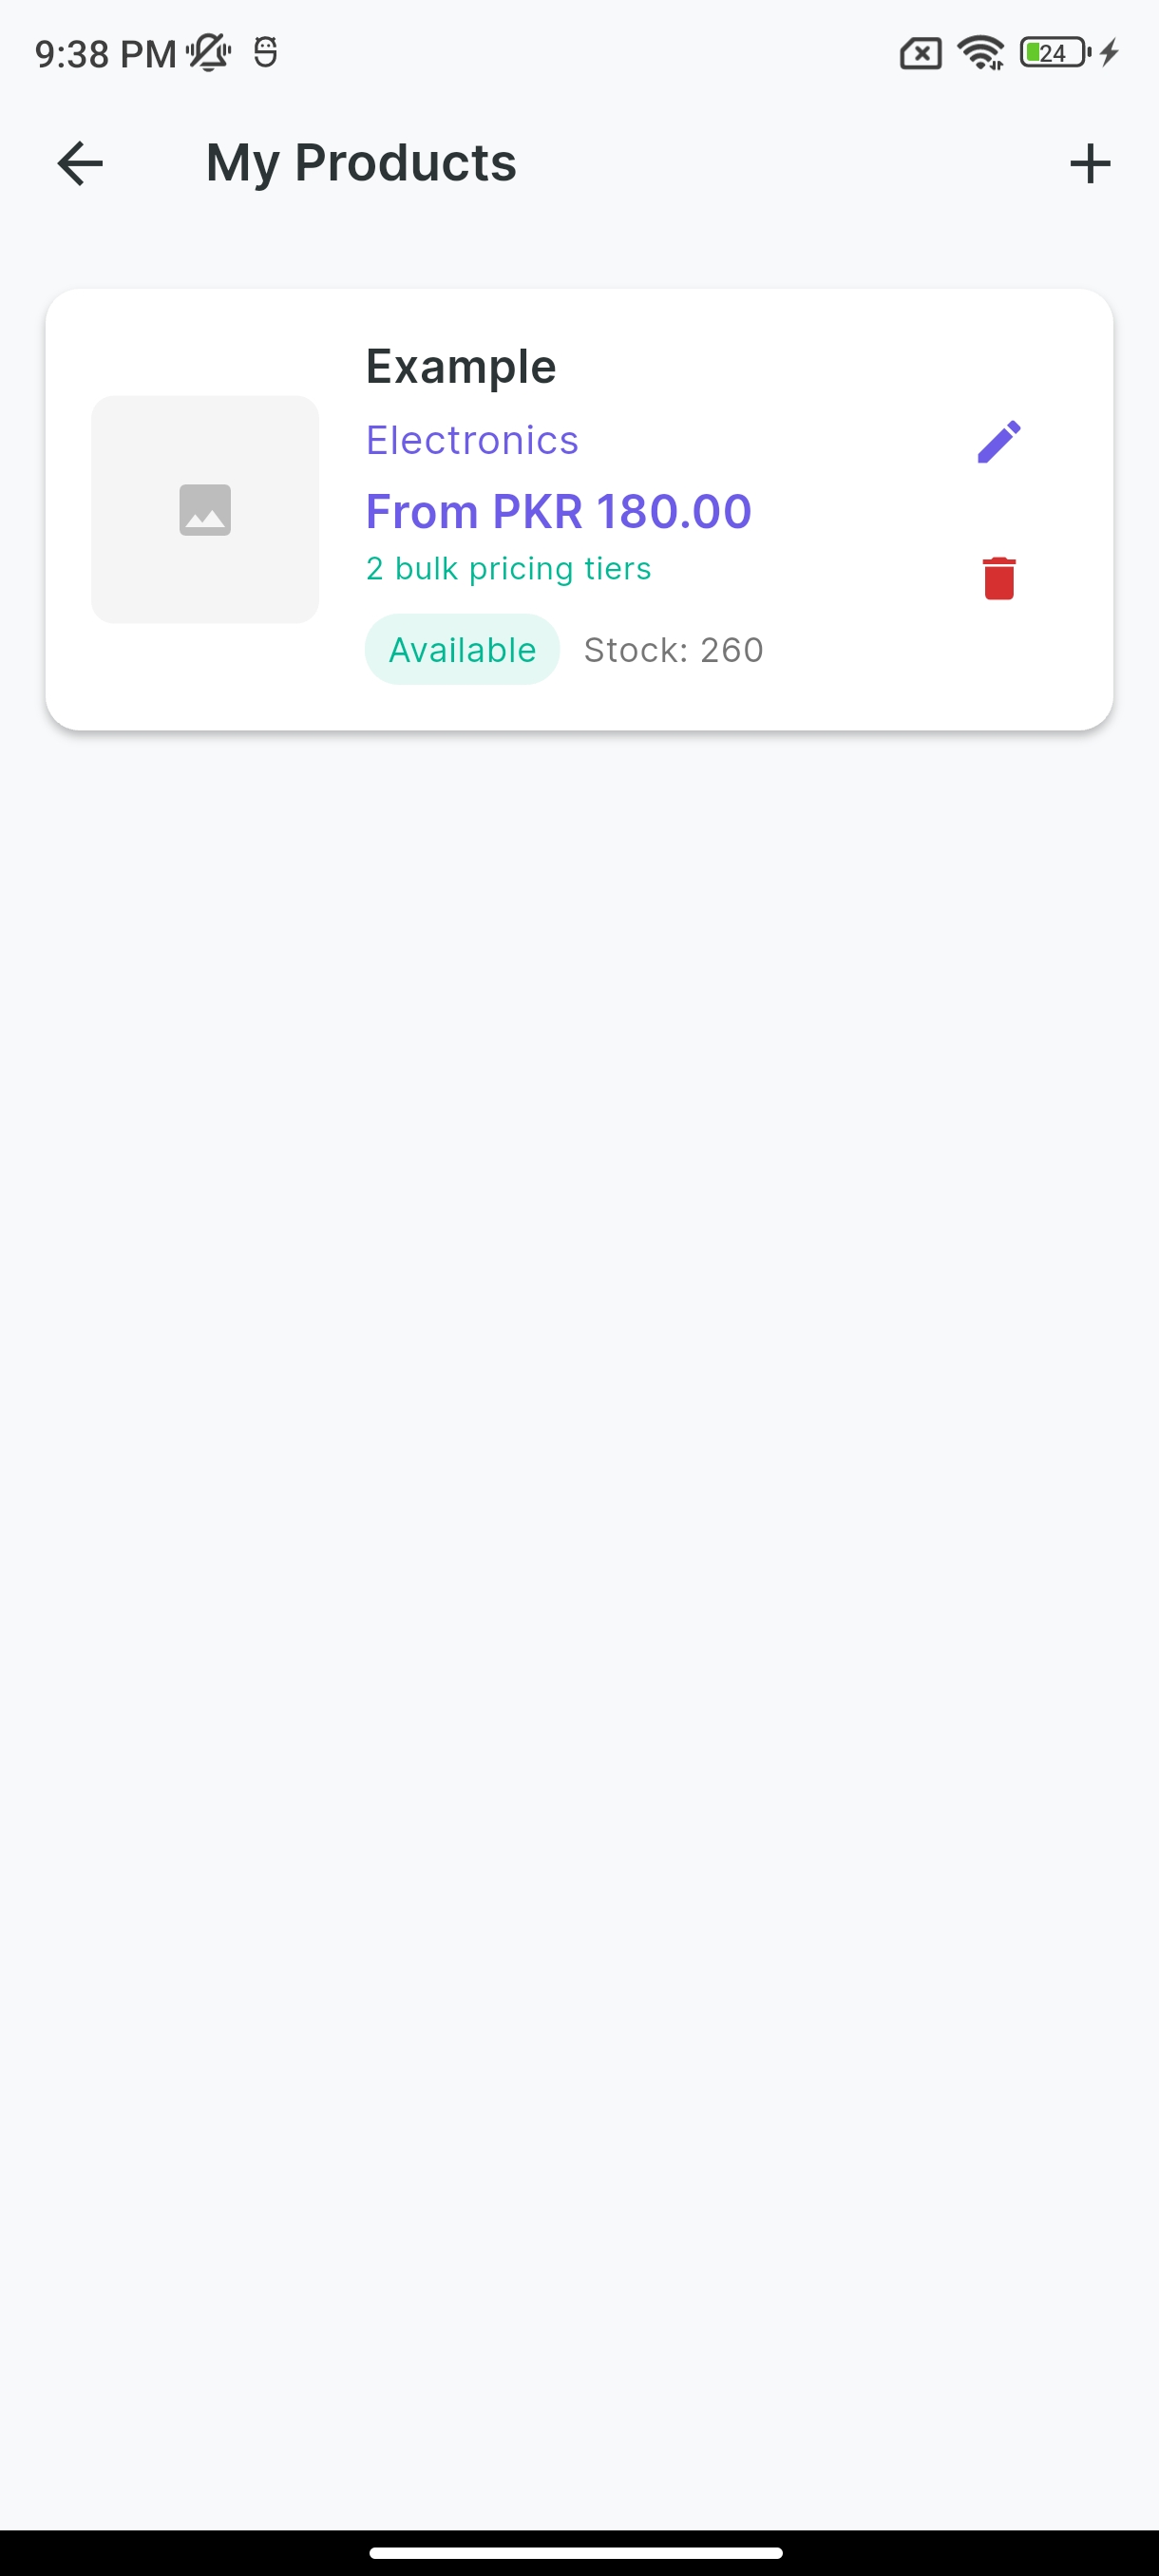
\includegraphics[width=0.4\textwidth]{figures/pictures project/sellerside/my products.jpeg}
\caption{My Products Screen Interface}
\label{fig:admindashboard2}
\end{figure}

The product listing screen of the seller is displayed in figure \ref{fig:admindashboard2}. It shows the items that have already been added by the seller in a tabular format to enable catalogue entries to be checked and edited effectively. This screen helps in the continued maintenance of the storefront inventory of the seller. After publishing products, sellers require an efficient method of checking their catalogue to ensure that their listings are correct and that they are live. The screen fulfils this role by sorting the items on display into a more management-friendly presentation as opposed to a customer-focused one. This type of listing interface can be employed to monitor stock display, pricing confirmation, and to determine products that might require modification or elimination. It also makes repetitive administrative works easier because it provides sellers with an overview of their merchandise. With a dynamic market place, buyers need to trust the product and make transactions, thus its quality and correctness is paramount. This display thus helps in catalogue governance on the seller side. It serves as an internal product browsing experience that corresponds to the external product browsing experience.

\begin{figure}[H]
\centering
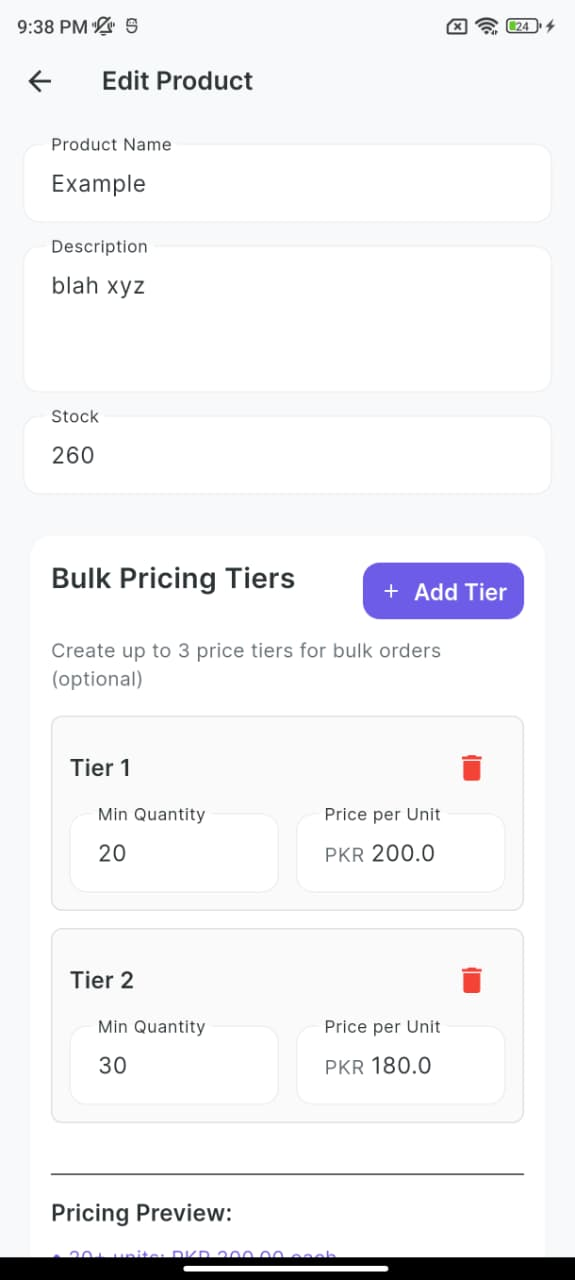
\includegraphics[width=0.4\textwidth]{figures/pictures project/sellerside/edit products.jpeg}
\caption{Edit Product Screen Interface}
\label{fig:admindashboard3}
\end{figure}

Figure \ref{fig:admindashboard3} displays the product editing screen that sellers use to edit existing listings. Using this interface, sellers have the ability to update product attributes, pricing details, among others without the need to create a new record. This enhances the flexibility of the catalogue and makes product maintenance easy. Editing of products once they are created is significant since commercial information tends to vary with time, particularly in competitive wholesale set-ups. As the market conditions vary, sellers might be required to change the prices, descriptions, stocks, or to fix the listing errors. The continuity of an existing product record is maintained by having an editing interface, and operational updates are easily made. This minimises duplication of the database and needless recreation of catalogue records. Usability wise, it also reduces maintenance effort as it maintains the tasks of modification in a familiar form based environment. The screen thus aids in data consistency, catalogue accuracy and responsiveness of the sellers. It is directly related to the sustainability of the marketplace inventory.

\begin{figure}[H]
\centering
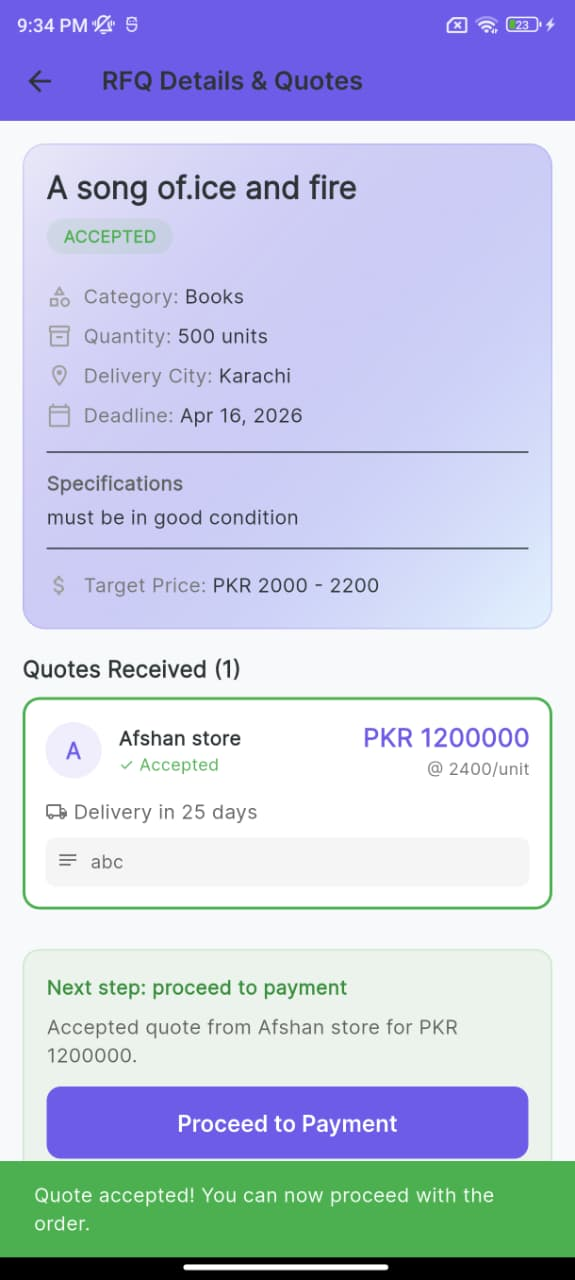
\includegraphics[width=0.4\textwidth]{figures/pictures project/sellerside/rfq details.jpeg}
\caption{RFQ Details Screen Interface}
\label{fig:users}
\end{figure}

As shown in figure \ref{fig:users}, the RFQ details screen is as shown by the seller side. It reveals the information on quotation requests by the customer in a detailed manner, which enables the seller to examine the requirements prior to writing a commercial response. This screen assists in making informed and correct quotation preparation. In B2B procurement, the quality of the submitted quote directly depends on the skills of a seller to interpret customer needs in the appropriate manner. Detailed view is thus important since it offers the entire picture of the request instead of a summary of the marketplace. Quantity, delivery location, target price expectation and descriptive requirements are some of the information that can be used by the seller to determine feasibility and trade-level viability. Such a more detailed background diminishes the possibility of unrealistic or partial quotes. It also gives the seller the capability of matching the offer made with the expectations and operational limitations of the customer. This screen enhances the quality of negotiation in the platform by acting as an analytical step prior to submitting a quote. It is thus an important support interface to the RFQ process.
\begin{figure}[H]
\centering
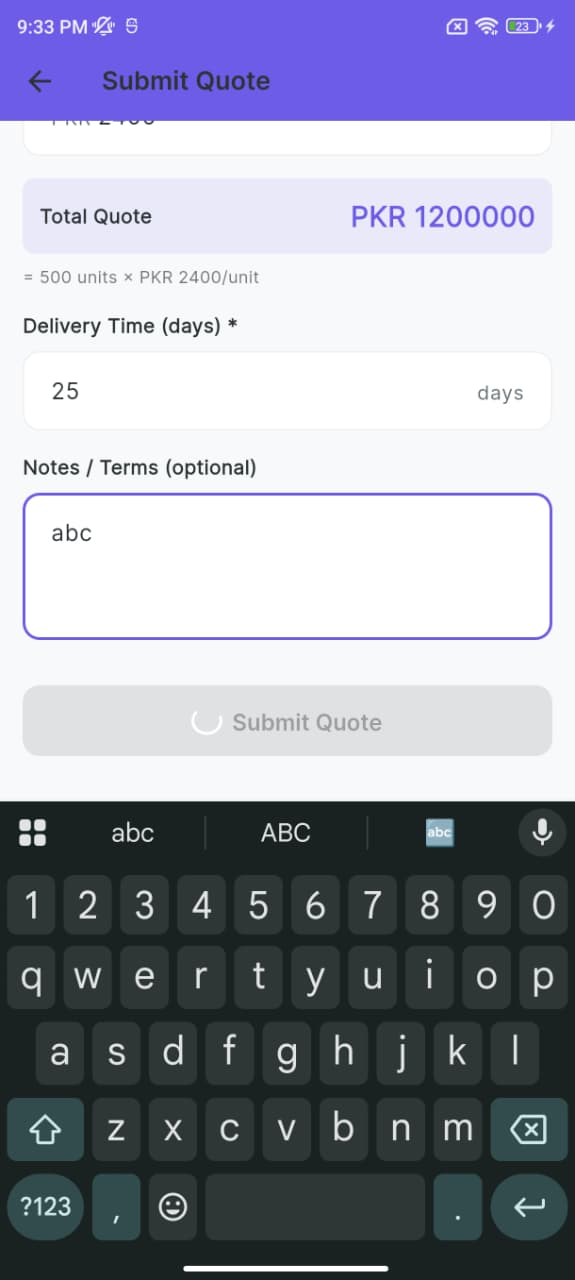
\includegraphics[width=0.4\textwidth]{figures/pictures project/sellerside/submit qouta.jpeg}
\caption{Submit Quote Screen Interface}
\label{fig:appointments}
\end{figure}

Figure \ref{fig:appointments} illustrates the quote submission interface that sellers use in response to an RFQ. The screen records the quoted price, delivery schedule and any notes or conditions that are optional allowing the seller to make a full offer to the requesting customer. It is an important component of the quotation-based negotiation process. The interface will convert the intent of the seller into a structured commercial proposal, which can be assessed by the buyer. The incorporation of the financial and logistical sphere allows preparing the offers in a more realistic and practical manner than a bare price-only response. Optional notes provide sellers with space to provide information about assumptions, terms, or details of the services that can be considered during acceptance. The fact that there is a final submission action makes the quotation process in the system formal. Process wise, this screen will translate RFQ review to a tangible marketplace response. It also normalises the formatting of quotes among the sellers and this simplifies comparison among buyers. By doing so, the screen will not only add value to the quality of the negotiation but also to the consistency of transactions.


\begin{figure}[H]
\centering
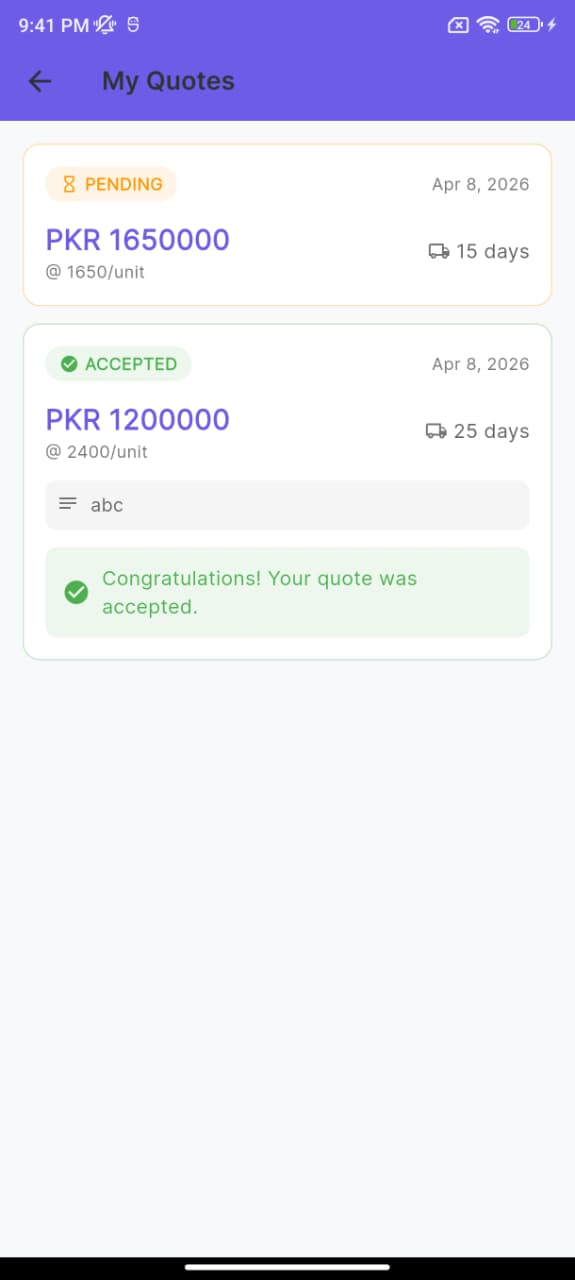
\includegraphics[width=0.4\textwidth]{figures/pictures project/sellerside/my qoutas.jpeg}
\caption{My Quotes Screen Interface}
\label{fig:reports}
\end{figure}

Figure \ref{fig:reports} shows the seller quotes screen, with all quotations submitted in the past, able to be viewed in a single location. This interface assists the sellers to track their bids and track quoted opportunities at the market. It enhances transparency of the seller involvement in the RFQ. Once quotes have been received, the sellers need a clear picture of their pending and past responses so as to be able to control any follow-up measures. The screen offers such visibility, which is to bundle together quotations into one management view. This assists the sellers in knowing how effectively they are working with customer demands and what possibilities they still have. A centralised quote list will also minimise the chances of losing track of already made offers in a busy business environment. In terms of usability, it forms continuity between the discovery of RFQs, the creation of quotes, and subsequent monitoring. This renders the quotation workflow complete as opposed to being fragmented on separate screens. The screen, therefore, plays a significant management role in the bid of the seller.

\begin{figure}[H]
\centering
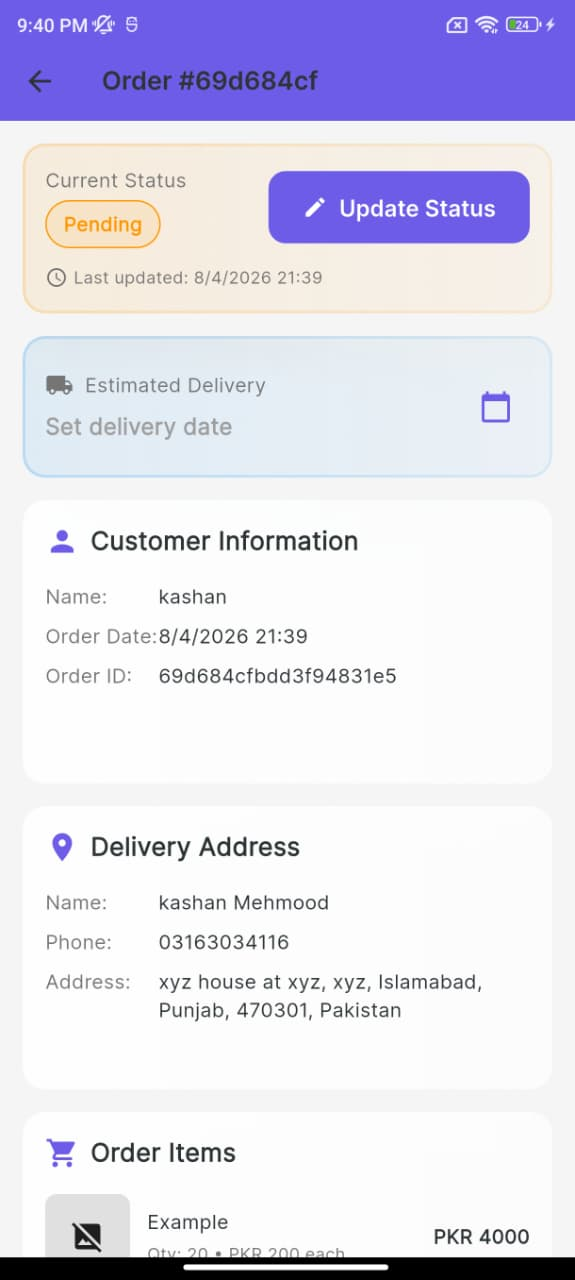
\includegraphics[width=0.4\textwidth]{figures/pictures project/sellerside/order info.jpeg}
\caption{Order Information Screen Interface}
\label{fig:submissions}
\end{figure}

The order information screen shown to sellers is shown in figure \ref{fig:submissions}. It is a more in-depth look at an order, enabling the seller to examine transaction data and information related to fulfilment prior to the next action in the business. This enhances seller-side processing and monitoring of orders. When the seller requires to establish what has been bought, expectations of delivery, or prepare status changes in the order lifecycle, detailed order checking is required. This screen aids those activities by showing an in-depth view of operation compared to the higher order list. The extra data assists in avoiding fulfilment errors and allows making the coordination with customer requirements more efficient. It is also used as a reference point in responding to order specific questions using the messaging channel. Practically, these detail views are very crucial in ensuring that an order is well handled particularly when there are many transactions being handled at once. The screen thus supplements the overall orders management interface by allowing closer viewing and preparedness to action. It has a direct effect on quality of service, accuracy of fulfilment and accountability of the seller.





